%% For double-blind review submission, w/o CCS and ACM Reference (max submission space)
\documentclass[sigplan,10pt,review,anonymous]{acmart}
\settopmatter{printfolios=true,printccs=false,printacmref=false}
%% For double-blind review submission, w/ CCS and ACM Reference
%\documentclass[sigplan,review,anonymous]{acmart}\settopmatter{printfolios=true}
%% For single-blind review submission, w/o CCS and ACM Reference (max submission space)
%\documentclass[sigplan,review]{acmart}\settopmatter{printfolios=true,printccs=false,printacmref=false}
%% For single-blind review submission, w/ CCS and ACM Reference
%\documentclass[sigplan,review]{acmart}\settopmatter{printfolios=true}
%% For final camera-ready submission, w/ required CCS and ACM Reference
%\documentclass[sigplan]{acmart}\settopmatter{}


%% Conference information
%% Supplied to authors by publisher for camera-ready submission;
%% use defaults for review submission.
\acmConference[]{}{}{}
\acmYear{}
\acmISBN{} % \acmISBN{978-x-xxxx-xxxx-x/YY/MM}
\acmDOI{} % \acmDOI{10.1145/nnnnnnn.nnnnnnn}
\startPage{1}

%% Copyright information
%% Supplied to authors (based on authors' rights management selection;
%% see authors.acm.org) by publisher for camera-ready submission;
%% use 'none' for review submission.
%\setcopyright{none}
%\setcopyright{acmcopyright}
\setcopyright{acmlicensed}
%\setcopyright{rightsretained}
%\copyrightyear{2018}           %% If different from \acmYear

%% Bibliography style
\bibliographystyle{ACM-Reference-Format}
%% Citation style
%\citestyle{acmauthoryear}  %% For author/year citations
%\citestyle{acmnumeric}     %% For numeric citations
%\setcitestyle{nosort}      %% With 'acmnumeric', to disable automatic
                            %% sorting of references within a single citation;
                            %% e.g., \cite{Smith99,Carpenter05,Baker12}
                            %% rendered as [14,5,2] rather than [2,5,14].
%\setcitesyle{nocompress}   %% With 'acmnumeric', to disable automatic
                            %% compression of sequential references within a
                            %% single citation;
                            %% e.g., \cite{Baker12,Baker14,Baker16}
                            %% rendered as [2,3,4] rather than [2-4].


%%%%%%%%%%%%%%%%%%%%%%%%%%%%%%%%%%%%%%%%%%%%%%%%%%%%%%%%%%%%%%%%%%%%%%
%% Note: Authors migrating a paper from traditional SIGPLAN
%% proceedings format to PACMPL format must update the
%% '\documentclass' and topmatter commands above; see
%% 'acmart-pacmpl-template.tex'.
%%%%%%%%%%%%%%%%%%%%%%%%%%%%%%%%%%%%%%%%%%%%%%%%%%%%%%%%%%%%%%%%%%%%%%


%% Some recommended packages.
\usepackage{booktabs}   %% For formal tables:
                        %% http://ctan.org/pkg/booktabs
\usepackage{subcaption} %% For complex figures with subfigures/subcaptions
                        %% http://ctan.org/pkg/subcaption
\usepackage{listings}
\usepackage{paralist}
\usepackage{tikz}
\usetikzlibrary{calc,patterns,decorations.pathmorphing,decorations.markings,shapes,arrows}
\usepackage{bbding} % for \checkmark
\usepackage{bbm}
\usepackage{mathrsfs}
\usepackage{adjustbox}
\usepackage{mathpartir,xparse}
\usepackage{mdframed}

\usepackage{nameref}

\usepackage{xspace}
\usepackage{verbatim}
\usepackage{epstopdf}
\usepackage{algorithm2e}

% General
\newcommand{\tb}[1]{\textbf{#1}}
\newtheorem{invariant}{Invariant}
\newtheorem{assumption}{Assumption}

\newcommand{\A}{\mathcal{A}}
\newcommand{\D}{\mathcal{D}}
\newcommand{\vs}{{\textbf{s}}}

\newcommand{\w}[1]{\ensuremath{\textit{#1}}}
\newcommand{\m}[1]{\ensuremath{\texttt{#1}}}
\newcommand{\s}[1]{\ensuremath{\textsf{#1}}}
\newcommand{\p}[1]{\ensuremath{\left(#1\right)}}
\newcommand{\pl}[1]{\ensuremath{\left\langle#1\right\rangle}}
\newcommand{\OR}{\mbox{ }|\mbox{ }}
\newcommand{\NMAX}{\mathit{N_{sys}}}
\newcommand{\st}{.\mbox{ }}
\newcommand{\finto}{\ensuremath{\stackrel{\mathtt{fin}}{\longrightarrow}}}
\newcommand{\defeq}{\ensuremath{\stackrel{\mathtt{def}}{=}}}
\newcommand{\cond}[1]{\ensuremath{\left\{\begin{array}{ll} #1 \end{array}\right.}}
\newcommand{\lst}[1]{\begin{itemize} {#1} \end{itemize}}
\newcommand{\pby}[1]{\hspace*{\fill}{#1}}
\newcommand{\slide}[2][]{ \begin{frame} \frametitle{#1} {#2} \end{frame} }
\newcommand{\etal}{\textit{et al.}\xspace}
\newcommand{\MW}{\sf{allwrite}}
\newcommand{\SW}{\sf{allread}}
\newcommand{\lgname}{\emph{K\kern-2pt oord}\xspace}
\newcommand{\toolname}{\emph{CyPhyHouse}\xspace}
\newcommand{\appname}{\emph{AppName}\xspace}
\newcommand{\UINS}{ID\xspace}
\newcommand{\kbmc}{\emph{KoordBMC}}
\newcommand{\kiic}{\emph{KoordProver}}
\newcommand{\ksem}{\emph{Koord Semantics}}
\newcommand{\sympost}{\emph{Symbolic Post Generation}}
\newcommand{\myuin}{\mathit{pid}\xspace}
\newcommand{\Var}{\mathit{Var}\xspace}
\newcommand{\Port}{\mathit{Port}\xspace}
\newcommand{\Event}{\mathit{Event}}

\newcommand{\Val}{\mathit{Val}\xspace}
\newcommand{\Cfield}{\mathit{Cfield}\xspace}

\newcommand{\cName}{\mathit{cName}\xspace}
\newcommand{\dmap}{{\sf DMap}\xspace}
\newcommand{\domain}{\mathit{domain}}

\newcommand{\End}{\mathit{End}\xspace}

\newcommand{\Post}{\mathit{Pe}\xspace}
\newcommand{\Final}{\mathit{Fn}\xspace}
%\newcommand{\Final}{\mathit{Final}\xspace}
\newcommand{\traj}{\mathit{traj}\xspace}
\newcommand{\pt}{\mathit{Pt}_{[0,\delta]}}
\newcommand{\ft}{\mathit{Pt}_\delta}
%evaluation property semantics
\newcommand{\eval}{\mathit{eval}}
\newcommand{\sat}{\rightarrow_\mathit{sat}}
\newcommand{\frontier}{\mathit{Fr}}
\newcommand{\Reach}{\mathit{Rc}}
% For references
\newcommand{\fig}[1]{Figure~\ref{#1}}
\newcommand{\lem}[1]{Lemma~\ref{#1}}
\newcommand{\asum}[1]{Assumption~\ref{#1}}
\newcommand{\portasum}{port assumption}
\newcommand{\inv}[1]{Invariant~\ref{#1}}
\newcommand{\theo}[1]{Theorem~\ref{#1}}
\newcommand{\coro}[1]{Corollary~\ref{#1}}
\newcommand{\defn}[1]{Definition~\ref{#1}}
\newcommand{\rmrk}[1]{Remark~\ref{#1}}
\newcommand{\myexample}[1]{Example~\ref{#1}}
\newcommand{\sect}[1]{$\S$~\ref{#1}}
\newcommand{\refsect}[1]{Section~\ref{sec:#1}}
\newcommand{\reffig}[1]{Figure~\ref{fig:#1}}
\newcommand{\refalg}[1]{Algorithm~\ref{#1}}

\newcommand{\ev}{\mathit{ev}}
\definecolor{orange}{rgb}{1,0.5,0}
\definecolor{darkgreen}{rgb}{0.0, 0.5, 0.0}
\newcommand{\marker}[1]{} %{\note{orange}{{#1}}}
\newcommand{\SM}[1]{\note{darkgreen}{SM: {#1}}}
\newcommand{\RG}[1]{\note{orange}{RG: {#1}}}
\newcommand{\logicarg}[2]{% \logicarg{<premise>}{<conclusion>}
  \begin{tabular}[t]{@{}c@{}}
    #1 \\ \hline #2
  \end{tabular}%
}
\newcommand{\sayan}[1]{\textcolor{blue}{#1}}
\newcommand{\rg}[1]{\textcolor{red}{#1}}
\newcommand{\chiao}[1]{\textcolor{green}{#1}}
\newcommand{\two}[4]{
	\parbox{.98\columnwidth}{\vspace{1pt} \vfill
		\parbox[t]{#1\columnwidth}{#3}%
		\hspace{.5cm}
		\parbox[t]{#2\columnwidth}{#4}%
	}}
\newcommand{\three}[5]{
	\parbox{.98\columnwidth}{\vspace{1pt} \vfill
		\parbox[t]{#1\columnwidth}{#3}%
		\hspace{.5cm}
		\parbox[t]{#2\columnwidth}{#4}%\vfill
				\hspace{.5cm}
		\parbox[t]{#2\columnwidth}{#5}%
	}}
	
\lstdefinelanguage{Koord}{
    basicstyle=\scriptsize,
    identifierstyle=\it,
    mathescape=true,
    tabsize=20,
    sensitive=false,
    columns=fullflexible,
    keepspaces=true,
    flexiblecolumns=true,
    basewidth=0.05em,
    moredelim=[il][\rm]{//},
    moredelim=[is][\bf ]{*}{*},
    keywordstyle=[1]\bf,
    keywords=[1]{
        and, agent, actuator, actuators, allread, allwrite, atomic, assume,
        break,
        def,
        eff, else, elseif, end,
        for, foreach, forget,
        if, import, in, init, input, internal, invariant,
        local,
        module,
        or,
        pre,
        return,
        sensor, sensors, stop,
        then, type, thread, to,
        using,
        variables, vocabulary,
        when, where, while, with},
    keywordstyle=[2]\it\color{olive},
    keywords=[2]{
        bool,
        int,
        list,
        pathplanner, point,
        set,
        task},
    keywordstyle=[3]\it\color{brown},
    keywords=[3]{
        false,
        len,
        pid,
        true},
    literate=
    {(}{{$($}}1
    {)}{{$)$}}1
    % LaTeX math symbols
    {\\in}{{$\in\ $}}1
    {\\preceq}{{$\preceq\ $}}1
    {\\subset}{{$\subset\ $}}1
    {\\subseteq}{{$\subseteq\ $}}1
    {\\supset}{{$\supset\ $}}1
    {\\supseteq}{{$\supseteq\ $}}1
    {\\forall}{{$\forall$}}1
    {\\le}{{$\le\ $}}1
    {\\ge}{{$\ge\ $}}1
    {\\gets}{{$\gets\ $}}1
    {\\cup}{{$\cup\ $}}1
    {\\cap}{{$\cap\ $}}1
    {\\langle}{{$\langle$}}1
    {\\rangle}{{$\rangle$}}1
    {\\exists}{{$\exists\ $}}1
    {\\bot}{{$\bot$}}1
    {\\rip}{{$\rip$}}1
    {\\emptyset}{{$\emptyset$}}1
    {\\notin}{{$\notin\ $}}1
    {\\not\\exists}{{$\not\exists\ $}}1
    {\\ne}{{$\ne\ $}}1
    {\\to}{{$\to\ $}}1
    {\\implies}{{$\implies\ $}}1
    % LSL symbols (one-character)
    {<*>}{{$\langle*\rangle$}}1
    {=}{{$=$}}1
    {~}{{$\neg\ $}}1
    {|}{{$\mid$}}1
    {'}{{$^\prime$}}1
    % LSL symbols (two characters)
    {\\A}{{$\forall\ $}}1
    {\\E}{{$\exists\ $}}1
    {\\/}{{$\vee\,$}}1
    {\\vee}{{$\vee\,$}}1
    {/\\}{{$\wedge\,$}}1
    {\\wedge}{{$\wedge\,$}}1
    {=>}{{$\Rightarrow\ $}}1
    {->}{{$\rightarrow\ $}}1
    {<=}{{$\ \leq\ $}}1
    {<-}{{$\leftarrow\ $}}1
    {==}{{$=\mathrel{\mkern-3mu}=$}}2
    {<=}{{$\leq$}}1
    {>=}{{$\geq$}}1
    {~=}{{$\neq\ $}}1
    {\\U}{{$\cup\ $}}1
    {\\I}{{$\cap\ $}}1
    {|-}{{$\vdash\ $}}1
    {-|}{{$\dashv\ $}}1
    {<<}{{$\ll\ $}}2
    {>>}{{$\gg\ $}}2
    {||}{{$\|$}}1
    {\\<}{{$\langle$}}1
    {\\>}{{$\rangle$}}1
    {[}{{$[$}}1
    {]}{{$]$}}1
    {<=>}{{$\Leftrightarrow\ $}}2
    {<->}{{$\leftrightarrow\ $}}2
    {(+)}{{$\oplus\ $}}1
    {(-)}{{$\ominus\ $}}1
    {_i}{{$_{i}$}}1
    {_j}{{$_{j}$}}1
    {_{i,j}}{{$_{i,j}$}}3
    {_{j,i}}{{$_{j,i}$}}3
    {_0}{{$_0$}}1
    {_1}{{$_1$}}1
    {_2}{{$_2$}}1
    {_n}{{$_n$}}1
    {_k}{{$_n$}}1
    %        {-}{{$\ms{-}$}}1
    {@}{{}}0
    {\\delta}{{$\delta$}}1
    {\\R}{{$\R$}}1
    {\\Rplus}{{$\Rplus$}}1
    {\\N}{{$\N$}}1
    {\\times}{{$\times\ $}}1
    {\\tau}{{$\tau$}}1
    {\\alpha}{{$\alpha$}}1
    {\\beta}{{$\beta$}}1
    {\\gamma}{{$\gamma$}}1
    {\\ell}{{$\ell\ $}}1
    {--}{{$-\ $}}1
    {\\TT}{{\hspace{1.5em}}}3
}
	
	
	\lstdefinelanguage{NumKoord}[]{Koord}
	{
		numbers=left,
		numbersep=15pt,
		numberstyle=\tiny,
		stepnumber=1,
		numbersep=4pt,
	}
	
	\lstdefinelanguage{KoordNum}[]{Koord}
	{
		numbers=right,
		numbersep=15pt,
		numberstyle=\tiny,
		stepnumber=1,
		numbersep=4pt,
	}


% numbers sets

\newcommand{\nnt}{{\sf T}^{\geq 0}}             %nonnegative time points
\newcommand{\post}{{\sf T}^{>0}}                %positive time points
\newcommand{\Variables}{{\sf V}}                %variables

\newcommand{\num}[1]{\relax\ifmmode \mathbb #1\else $\mathbb #1$\fi}
\newcommand{\nnnum}[1]{\relax\ifmmode 
	{\mathbb #1}_{\geq 0} \else ${\mathbb #1}_{\geq 0}$
	\fi}
\newcommand{\npnum}[1]{\relax\ifmmode 
	{\mathbb #1}_{\leq 0} \else ${\mathbb #1}_{\leq 0}$
	\fi}
\newcommand{\pnum}[1]{\relax\ifmmode 
	{\mathbb #1}_{> 0} \else ${\mathbb #1}_{> 0}$
	\fi}
\newcommand{\nnum}[1]{\relax\ifmmode 
	{\mathbb #1}_{< 0} \else ${\mathbb #1}_{< 0}$
	\fi}
\newcommand{\plnum}[1]{\relax\ifmmode 
	{\mathbb #1}_{+} \else ${\mathbb #1}_{+}$
	\fi}
\newcommand{\nenum}[1]{\relax\ifmmode 
	{\mathbb #1}_{-} \else ${\mathbb #1}_{-}$
	\fi}
\newcommand{\K}{$\mathbb{K}\ $}
\newcommand{\reals}{{\num R}}                    %reals
\newcommand{\booleans}{{\num B}}                    %reals
\newcommand{\nnreals}{{\nnnum R}}                    %nonnegative reals
\newcommand{\realsinfty}{{\num R} \cup \{\infty, -\infty\}}                    %nonnegative reals
\newcommand{\plreals}{{\plnum R}}                    %positive reals
\newcommand{\naturals}{{\num N}}                      %natural numbers
\newcommand{\integers}{{\num Z}}                      %integers
\newcommand{\rationals}{{\num Q}}                      %rationals
\newcommand{\nnrationals}{{\nnnum Q}}                   % nonnegative rationals
\newcommand{\Time}{{\num T}}  



%% Sasa, commenting commands:

\definecolor{WowColor}{rgb}{.75,0,.75}
\definecolor{SubtleColor}{rgb}{0,0,.50}
\definecolor{TODOColor}{rgb}{0,.50,0}

% inline
%\newcommand{\NA}[1]{#1}
\newcommand{\NA}[1]{\textcolor{SubtleColor}{ {\tiny \bf ($\star$)} #1}}
\newcommand{\TODO}[1]{\textcolor{TODOColor}{ {\tiny \bf TODO:} #1}}
\newcommand{\LATER}[1]{\textcolor{SubtleColor}{ {\tiny \bf ($\dagger$)} #1}}
\newcommand{\TBD}[1]{\textcolor{SubtleColor}{ {\tiny \bf (!)} #1}}
\newcommand{\PROBLEM}[1]{\textcolor{WowColor}{ {\bf (!!)} {\bf #1}}}
\newcommand{\ST}[1]{ \textcolor{SubtleColor}{ {\tiny \bf (!!)} \sout{#1} } }

%semantic macros
\newcommand{\pid}{\mathit{pid}}
\newcommand{\en}{\mathit{en}}
\newcommand{\ur}{\mathit{ur}}
\newcommand{\cp}{\mathit{cp}}
\newcommand{\turn}{\mathit{turn}}
\newcommand{\gconfig}{\mathcal{C}} %global config 
\newcommand{\lset}{L} %set of agent configurations 
\newcommand{\lconfig}[1]{L_{#1}} %configuration of agent i
\newcommand{\agnt}{L}
\newcommand{\pwg}{\mathbb{C}} %all possible global configs, (power set of)
\newcommand{\pwl}{\mathbbm{L}} %all possible local configs
\newcommand{\pwe}{\mathbb{E}} %all possible expressions. 
\newcommand{\pws}{\mathbb{S}} %all possible global context
\newcommand{\pwstmt}{\mathbb{S\mathit{tmt}}} %all possible statements

%%transition rules
\newcommand{\exprule}{\rightarrow_E\xspace}
\newcommand{\stmtrule}{\rightarrow_\mathit{Stmt}\xspace}
\newcommand{\sysrule}{\rightarrow_\mathit{Env}\xspace}
\newcommand{\progtrans}{\rightarrow_\mathit{prog}\xspace}
\newcommand{\envtrans}{\rightarrow_\mathit{env}\xspace}
%%semantic rule references 
\newcommand{\runrule}{Rule \textsc{run-sys}}
\newcommand{\et}{Rule \textsc{env-trans}\xspace}
\newcommand{\etp}{Rule \textsc{agent-env-to-prog}\xspace}
\newcommand{\getp}{Rule \textsc{env-to-prog}\xspace}
%\newcommand{\envrule}{Rule \textsc{}\xspace}
\newcommand{\eskip}{Rule \textsc{enskip-evnt}\ }
\newcommand{\edo}{Rule \textsc{en-evnt}\xspace}
\newcommand{\urdo}{Rule \textsc{ur-evnt}\xspace}
% as margin notes
\newcounter{margincounter}
\newcommand{\displaycounter}{{\arabic{margincounter}}}
\newcommand{\incdisplaycounter}{{\stepcounter{margincounter}\arabic{margincounter}}}
\newcommand{\env}{\mathtt{env}}
\newcommand{\prog}{\mathtt{prog}}



\newcommand{\fTBD}[1]{\textcolor{SubtleColor}{$\,^{(\incdisplaycounter)}$}\marginpar{\tiny\textcolor{SubtleColor}{ {\tiny $(\displaycounter)$} #1}}}
\newcommand{\fTODO}[1]{\textcolor{TODOColor}{$\,^{(\incdisplaycounter)}$}\marginpar{\tiny\textcolor{TODOColor}{ {\tiny TODO $(\displaycounter)$}:  #1}}}

\newcommand{\fPROBLEM}[1]{\textcolor{WowColor}{$\,^{((\incdisplaycounter))}$}\marginpar{\tiny\textcolor{WowColor}{ {\bf $\mathbf{((\displaycounter))}$} {\bf #1}}}}

\newcommand{\fLATER}[1]{\textcolor{SubtleColor}{$\,^{(\incdisplaycounter\dagger)}$}\marginpar{\tiny\textcolor{SubtleColor}{ {\tiny $(\displaycounter\dagger)$} #1}}}
\newcommand{\mytitle}{Working Title}
\newcommand{\qfunc}{\mathit{quant}}
\newcommand{\qinv}{\mathit{quant}^{-1}}
\newcommand{\qdom}{\mathit{Q}}
\newcommand{\map}{\mathit{map}}
\newcommand{\world}{\mathit{world}}
\newcommand{\pos}{\mathit{pos}}
\newcommand{\mapprob}{\mathit{Map2D}}
\newcommand{\sensarea}{\mathit{sa}}
\newcommand{\lmap}{\mathit{localMap}}
\newcommand{\gmap}{\mathit{map}}
\newcommand{\ff}{\mathit{frontier}}
\newcommand{\qdfunc}{quantized domain function}
\newcommand{\sensfunc}{\mathit{scanToMap}}
\newcommand{\rmap}{\mathit{ws}}
\newcommand{\Access}{\mathit{access}}
\newcommand{\ps}{\mathit{ps}}


\begin{document}

%% Title information
\title{\lgname: a language for distributed robotics}         %% [Short Title] is optional;
                                        %% when present, will be used in
                                        %% header instead of Full Title.
%\titlenote{with title note}             %% \titlenote is optional;
                                        %% can be repeated if necessary;
                                        %% contents suppressed with 'anonymous'
%\subtitle{Subtitle}                     %% \subtitle is optional
%\subtitlenote{with subtitle note}       %% \subtitlenote is optional;
                                        %% can be repeated if necessary;
                                        %% contents suppressed with 'anonymous'


%% Author information
%% Contents and number of authors suppressed with 'anonymous'.
%% Each author should be introduced by \author, followed by
%% \authornote (optional), \orcid (optional), \affiliation, and
%% \email.
%% An author may have multiple affiliations and/or emails; repeat the
%% appropriate command.
%% Many elements are not rendered, but should be provided for metadata
%% extraction tools.

%% Author with single affiliation.
\author{First1 Last1}
\authornote{with author1 note}          %% \authornote is optional;
                                        %% can be repeated if necessary
\orcid{nnnn-nnnn-nnnn-nnnn}             %% \orcid is optional
\affiliation{
  \position{Position1}
  \department{Department1}              %% \department is recommended
  \institution{Institution1}            %% \institution is required
  \streetaddress{Street1 Address1}
  \city{City1}
  \state{State1}
  \postcode{Post-Code1}
  \country{Country1}                    %% \country is recommended
}
\email{first1.last1@inst1.edu}          %% \email is recommended

%% Author with two affiliations and emails.
\author{First2 Last2}
\authornote{with author2 note}          %% \authornote is optional;
                                        %% can be repeated if necessary
\orcid{nnnn-nnnn-nnnn-nnnn}             %% \orcid is optional
\affiliation{
  \position{Position2a}
  \department{Department2a}             %% \department is recommended
  \institution{Institution2a}           %% \institution is required
  \streetaddress{Street2a Address2a}
  \city{City2a}
  \state{State2a}
  \postcode{Post-Code2a}
  \country{Country2a}                   %% \country is recommended
}
\email{first2.last2@inst2a.com}         %% \email is recommended
\affiliation{
  \position{Position2b}
  \department{Department2b}             %% \department is recommended
  \institution{Institution2b}           %% \institution is required
  \streetaddress{Street3b Address2b}
  \city{City2b}
  \state{State2b}
  \postcode{Post-Code2b}
  \country{Country2b}                   %% \country is recommended
}
\email{first2.last2@inst2b.org}         %% \email is recommended


%% Abstract
%% Note: \begin{abstract}...\end{abstract} environment must come
%% before \maketitle command
\begin{abstract}
% Why
A program for a robot in an ensemble has to interact with its physical environment using sensors and actuators, and with other robots, using over a network, in addition to implementing the control and coordination algorithm. While various impressive applications have been demonstrated with robotic ensembles, developing, debugging, and testing these applications typically require months to years. Developing these applications require detailed knowledge of control theory, path planning, network protocols, and various platform specific details. The languages and tools used to develop robot programs provide no portability of code across platforms. 

Koord is a domain-specific language for distributed robotics applications. It separates the platform-independent control and coordination code from platform-specific concerns of sensing, communication, and low-level  control.
Koord raises the level of abstraction in programming  by providing distributed shared memory for coordination;
it allows parameterized controllers for portability across different physical platforms,
and it is based on a familiar event-triggered concurrent programming model.
We present the formal semantics of Koord in the \K executable semantic framework.
This narrows the gap between the theoretical model of \lgname and its implementation and allows \sayan{formal reasoning/BMC}.
We present an implementation of \lgname that generates executable Python code, which has been deployed on robotic platforms.
Finally, we introduce a high-fidelity simulator and show how it can be used to test, visualize, and debug large deployments of \lgname applications.  
We illustrate the various features and the design decisions involved through applications such as platooning, formation flight, and distributed task allocation. \sayan{Statements about evaluation and hardware deployment.}
\end{abstract}


%% 2012 ACM Computing Classification System (CSS) concepts
%% Generate at 'http://dl.acm.org/ccs/ccs.cfm'.
\begin{CCSXML}
<ccs2012>
<concept>
<concept_id>10011007.10011006.10011008</concept_id>
<concept_desc>Software and its engineering~General programming languages</concept_desc>
<concept_significance>500</concept_significance>
</concept>
<concept>
<concept_id>10003456.10003457.10003521.10003525</concept_id>
<concept_desc>Social and professional topics~History of programming languages</concept_desc>
<concept_significance>300</concept_significance>
</concept>
</ccs2012>
\end{CCSXML}

\ccsdesc[500]{Software and its engineering~General programming languages}
\ccsdesc[300]{Social and professional topics~History of programming languages}
%% End of generated code


%% Keywords
%% comma separated list
\keywords{keyword1, keyword2, keyword3}  %% \keywords are mandatory in final camera-ready submission


%% \maketitle
%% Note: \maketitle command must come after title commands, author
%% commands, abstract environment, Computing Classification System
%% environment and commands, and keywords command.
\maketitle


\section{Introduction}
\label{sec:intro}

\paragraph{Motivation}
Programming systems that interact with physical processes are central in  robotics, manufacturing, IoT, and other cyberphysical systems. Typical domain specific languages (DSL) for these systems are platform specific and they combine  low-level sensing, communication, and control tasks with the application-level logic~\cite{nordmann2014robotics}. This  tight-coupling of applications with platform-specific details can hinder development, modularity, portability, code reuse, and testing. 

This need for raising the level of abstraction and separating the \emph{platform-independent} from the \emph{platform-dependent} concerns motivates our work. For example, consider an application for distributed package delivery with mobile robots in a building. The higher-level coordination has to deal with assigning robots to visit way-points in different rooms, load-balancing, and handling failures.  For all of the reasons mentioned above, these coordination tasks {\em should be\/} separated from the  steering control of the individual vehicles, indoor positioning, and message-level communication protocols tied to the specific hardware platforms. 

Current programming languages do not natively support such abstractions for programming distributed cyberphysical systems.  The developer will have to keep track of communication between different sensors, actuators, and program variables. The {\em robotic operating system (ROS)}~\cite{rosbridge_suite,ros} does provide useful libraries and  publish-subscribe messaging standards, but these are not integrated in a programming abstraction. Similarly, coordination across multiple robots has to be built from the ground up using message passing threads. In order to simulate and test the application, one has to create different threads or instances for the developed code corresponding to different agents, and on top of that, the agent programs have to be harnessed in a physical world simulator with proper sensor and actuator models. In order to analyze correctness, one has to first define the semantics of the system. This  is again challenging  as  distributed cyber-physical systems have concurrency and data flows in multiple time-scales. 
%A further source of concern is the gap between the system model with iand the executable code that is actually . 

An ongoing, multi-year, project at our lab aims to address some of these challenges by designing, developing, and evaluating an open source programming system for distributed robotics. \footnote{Information about this project and the links to downloadable software will be made available to the reviewers upon request. We omit the information here for the sake of maintaining anonymity.} In this paper, we present the design and the implementation of the  {\em $\lgname$ language} and the supporting software tools, namely the compiler, the \K executable semantics, and the simulator. This forms the  core of this programming system. $\lgname$ programs have been deployed on F1/10 vehicles, quadcopter, and roombas, and the hardware deployment will be presented in a future article. 





%
%\begin{figure}[h!]
%\centering
%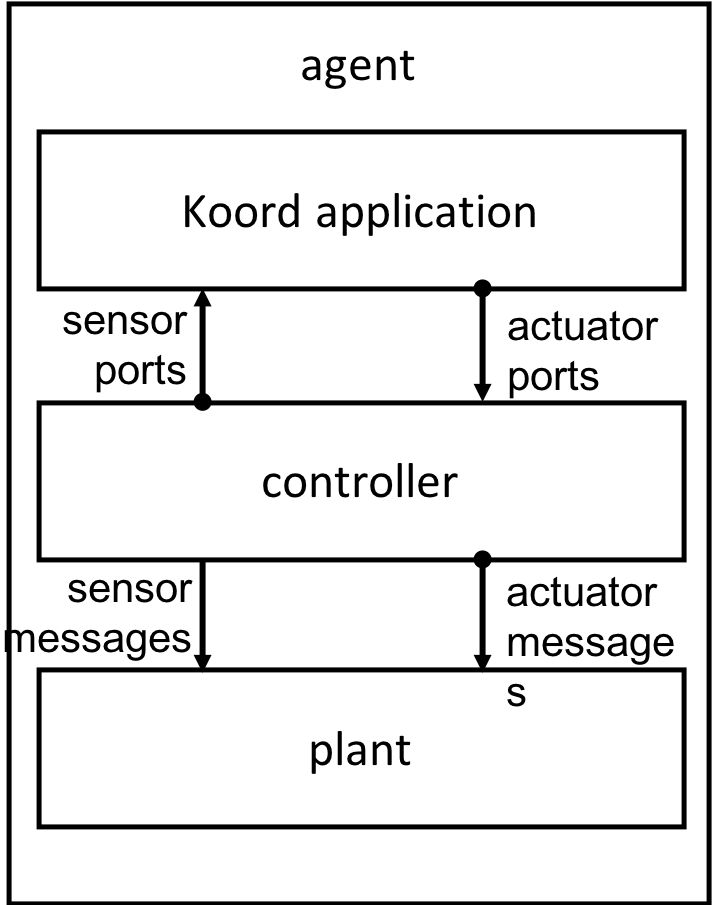
\includegraphics[width=0.48\textwidth]{figs/arch.png}
%\caption{\small CyPhyHouse framework. Major tools shown in blue.}
%\label{fig:arch}
%\end{figure}
%
\subsection{Contributions}
\subsubsection{Design and implementation of $\lgname$ language}
{\em We present a clean-slate design and implementation of an event-driven programming language, for distributed cyber-physical systems, namely $\lgname$.} 
%
$\lgname$ combines distributed shared memory abstraction for coordination across agents and a synchronous model of communication with the physical environment through sensors and actuators, all packed in a familiar precondition-effect style language.
%

Consider a simple line-formation program in which a set of $N$ robots form a equi-spaced line starting from arbitrary positions. The elementary algorithm is for each robot $i$ to repeatedly move towards the midpoint of the line joining the positions of $i-1$ and $i+1$. The extremal robots with ids $0$ and $N-1$ stay fixed. This is a archetypal protocol for synchronization, pattern formation, and consensus~\cite{Tsitsiklis:1986,Blondel,Magnusbook2010,Fax} in distributed robotics.
%
% \belowcaptionskip=-10pt
\begin{lstlisting}[label=lineform,caption=Lineform $\lgname$ program]
   using Motion:
      sensors pos psn
      actuators target
   allread: pos x $\label{lineformp}$
   TargetUpdate:
      pre True
      eff if not(pid == $\NMAX$ - 1 or pid == 0):
         Motion.target = mid(<x[pid+1],x[pid-1]>)
         x[pid] = Motion.psn
\end{lstlisting}

The above $10$ line  $\lgname$ program implements this line formation algorithm and can be simulated or deployed (see Figure~\ref{fig:shapeformplots1}). Among these $10$ lines of code, lines 1-5 import the {\em controller module\/} called {\em Motion\/} that enables this program to access the sensor port with the agent's position $(\mathit{psn})$ and the actuator port $(\mathit{target})$. An implementation of  a {\em controller module\/} has platform-specific path planners and low-level controllers for moving specific types of robots in the physical world. {\em Thus, with different implementations of the {\em Motion\/} interface the $\mathit{Lineform}$ $\lgname$  program can be ported to different platforms\/}. 

Another powerful feature of $\lgname$ used in the $\mathit{Lineform}$ program is the single-write multi-reader ({\bf allread}) shared array $x$, in which component $x[i]$ records the position of the $i^{th}$ robot in each round.  Shared variables allow the participating agents programs to coordinate without exposing the programmer to explicit message passing channels, buffers, and threads. This makes $\lgname$ programs succinct, readable, and often, as in the  above example, remarkably close to the textbook version of the algorithm. The $\lgname$ runtime system (discussed in more detail in Section~\ref{sec:software}) implements the propagation of  the shared variable write over messages. The formalization of the resulting semantics is discussed in Section~\ref{sec:K}.

%
The one and only event in the $\mathit{Lineform}$ program is $\mathit{TargetUpdate}$ (lines 5-9): it updates the target position of the agent  to be the midpoint of its neighbors.  Figure~\ref{fig:shapeformplots} shows the result of simulating a slightly modified version of $\mathit{Lineform}$ on the $\lgname$ simulator with $25$ robots forming a 3D-shape. The $\lgname$ compiler can also generate executables that can be deployed on several mobile robotic hardware platforms such as F1/10 cars~\cite{f1-10}, drones~\cite{}, and Roombas. 
%\renewcommand{\lstinputlisting}[1][]{\oldlstinputlisting[frame=lines,#1]}
 
%\begin{figure}[ht!]
%	\label{fig:lineform}
%	\noindent
%	\begin{center}
%		\scriptsize
%		\two{0.4}{0.6}
%		{\lstinputlisting[language=xyzNums,frame=lines]{code/lineform.tex}}
%	\par        
%	\end{center}
%	\caption{\small $\lgname$ program for line formation ({\em Left}) and its mathematical counterpart in robotics and control textbooks ({\em Right}).}
%\end{figure}

%The shared \emph{allread} variable $p$ (Line\ref{lineformp}) is used by the agents to communicate their position to the other robots. The function \emph{midpoint} is a part of the library functions provided for the data type \emph{pos}; where $$\mathit{midpoint}(p_1,p_2,\ldots,p_n) = pos(\frac{\Sigma_n p_i.x}{n},\frac{\Sigma_n p_i.y}{n},\frac{\Sigma_n p_i.z}{n}) $$.
%

%We have implemented a compiler for $\lgname$ that generates executable Python programs that can be either simulated in a discrete event simulator (discussed below) or 

\subsubsection{First formalization of a robotics or CPS language in \K}
% motivation
Implementations of programming languages usually contain many bugs. One common type of bugs creeps in from the gap between the official semantics of the language (as in a user manual) and the its implementation as embodied in a compiler. The \K framework~\cite{Kf} closes this gap by allowing the specification of {\em  formal executable semantics of any programming language} in terms of rewrite rules. These rewrite rules define how each and every possible statement in the  language changes, possibly nondeterministically, the ``state of the machine'' executing the program. 
%
\K  provided the most-complete-to-date formalization  of the C language~\cite{KC}. This semantics was tested against the GCC torture test suite and it successfully passed 99.2\% of 776 test programs~\cite{chuckythesis}. Recently, \K  was used to provide a formal semantics of x86-64~\cite{rusuadvepaper} and the Ethereum Virtual Machine (EVM) bytecode. 


%\K  using computations over states or configurations, and rewrite rules for said configurations. \K has several additional features including non deterministic execution, underspecification and explicit read-only and write only specifications for rewrite rules which makes \K suitable for defining concurrent and control intensive languages. 
{\em In order to close the above-mentioned gap, we have developed the complete executable formal semantics of $\lgname$ in \K.} This is the first formalization of a robotics or CPS language in \K;  and the first multi-agent language. \sayan{One challenge here is to define the ``state of the machine'' executing $\lgname$ programs. This state now has to include not only the states of the program variables of the different agents, but also the sensor and actuator ports, and the shared variables.}

\sayan{
Our key innovation for achieving this formalization is to parameterize the semantics with a set of {\em environment functions\/} that model the behavior of the physical environment, the controller, and other operations that are external to the application program.  The environment functions are called by the  back-end of \K to update certain state components (e.g., sensor and actuator ports). Thus, the formal semantics of $\lgname$ is also modular and portable across  different environment models. }

%ontroller behaviors with path-planners to the back-end of \K to specify rewrite rules for them, as the $\lgname$ language itself lets the user use predefined controller modules.
In addition, the shared memory semantics of $\lgname$ is implemented over  message passing.. \sayan{So what is challenging interesting in what we have done here? Mention synchronous round-by-round execution. Events. Shared memory propagation. }


Our \K implementation of $\lgname$ enables us to execute  programs \emph{semantically accurately}. So we can to design test suites for any implementation of the language semantics. 
\sayan{This is weak, as we have not done this.}
\sayan{Mention nondeterminism?}
To support formal analysis in case of non-specific initial states, we also implemented an interval arithmetic in \K, and support execution of $\lgname$ programs where the initial values of variables are provided in intervals. We implemented a explicit state bounded-model-checking  tool on top of the \K semantics to provide this additional feature. \sayan{What are the main conclusions of this part? Give pointer to section ahead.}

\sayan{Demonstration of feasibility?} 
\sayan{copied from before:
Design and development of the $\lgname$ programming language and the supporting $\mathbb{K}$-based~\cite{Kpaper} verification tool \kbmc\, are discussed here for the sake of completeness; those details will appear elsewhere~\cite{koordreport}.}

\subsubsection{$\lgname$ simulator and applications}

{\em We have developed a high-fidelity, multi-threaded simulator for $\lgname$ applications (\reffig{simulator}). } The simulator can execute instances with 50+ agents with heterogeneous dynamics, executing $\lgname$ applications, and therefore, is a powerful tool for debugging and performance analysis.  

The major challenges involved in designing a simulator were to create a simulation engine that exactly simulates the behavior expected on hardware deployment. 
\sayan{But this is on the surface an impossible task.}
To that end, the simulator uses motion automata, which can be provided any programmable dynamics to simulate the robot dynamics. The simulated sensed data can also be also provided realistic noises and dynamics to mimic actual system dynamics. The communication protocols to propagate shared memory messages between agents are also a part of the simulator communication module. The time between two computational steps (or discrete event loop iterations) is used to propagate messages to implement shared memory as in the actual hardware stack.

The simulator enables the user to test their discrete event loop with simple motion models to test and debug the application program logic without incurring the cost of hardware deployment in case of buggy programs. The simulator also serves as a visualization tool as it can be used to plot the behavior of any program variables, or controller variables. For instance, we implemented a robot \emph{formation} app in $\lgname$, where several robots form a shape in which they are evenly distributed.

\begin{figure}[h!]
\begin{minipage}{0.5\textwidth}
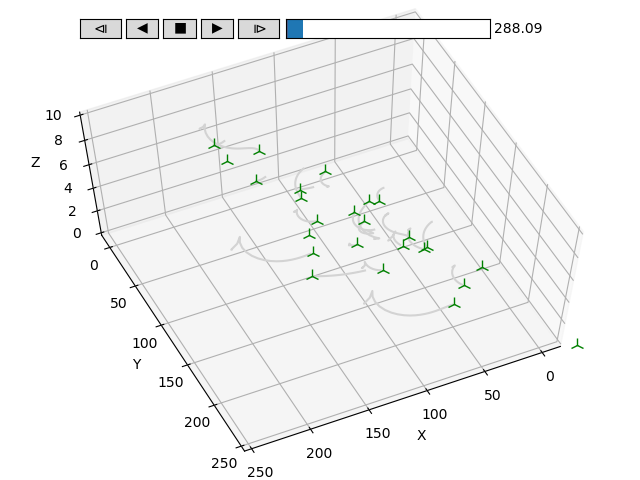
\includegraphics[width=.5\textwidth]{figs/formation1.png}\hfill
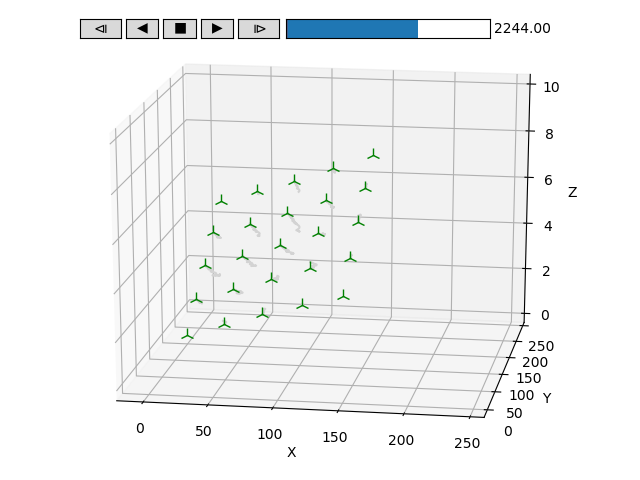
\includegraphics[width=.5\textwidth]{figs/formation4.png}\hfill%
%\includegraphics[width=.3\textwidth]{figs/Platooning_2.png}}\hfill%
\end{minipage}%
\caption{Screenshot of $\lgname$ simulator visualizing positions of a swarm of $25$ agents running a slightly modified version of $\mathit{Lineform}$ application forming a 3D-shape in space.}
\label{fig:shapeplots}
\end{figure}




%\subsubsection{Other by-products}


%Design and development of the CyPhyHouse open source software system. This includes a discrete event simulator for distributed robotic systems, the application launcher, the run-time logging and monitoring system, and an integrated indoor positioning system. All of these software tools are integrated with our new robot programming language called $\lgname$ and its compiler. 





%Design and development of the Koord programming language and the supporting verification tool KoordBMC~\cite{koordreport}--- significant, related but separate efforts---are not contributions of the current paper; we discuss their usage for the sake of completeness. 
% completely describing the framework. 
% the Demonstration of an example application development using CyPhyHouse tools and deployment on a physical system using multiple quadcopters.
%Non-contributions: Spell these out  to avoid misdirected criticisms and conflict with overlapping publications.
%\begin{itemize} 
%\item Language design
%\item Verification tools.
%\item Low-level controller design for vehicles.
%\end{itemize} 

%\begin{figure}[h!]
%\centering
%\includegraphics[width=0.45\textwidth]{figs/exp_traces.png}
%\caption{\small Experimental run in our testbed. The traces show the path of each robot for the last $2$ seconds. }
%\label{fig:exp_traces}
%\end{figure}

%
%%\footnote{\href{https://cyphyhouse.github.io/index.html}{https://cyphyhouse.github.io}}: an open source software framework for programming, rapid deployment, and testing of distributed robotics applications. 
%\sayan{The high-level $\lgname$ language enables users to write succinct distributed coordination applications without getting bogged down by messaging and thread management issues (See Examples in \reffig{lineform} and \reffig{taskapp}).}
%Using the CyPhyHouse framework around $\lgname$, a user can code, compile, launch, and run applications in a highly-automated fashion (\reffig{arch}). 
%\sayan{The framework has been built over three years and has more than 100k lines of source code.}


    
    \section{Related work}
    \label{sec:related}
    \sayan{Modern programming languages like C\# and Swift, and   compiler infrastructures like LLVM~\cite{llvm} have revolutionized the application development ecosystem in mobile computing.
%\paragraph*{D.} 
Inspired by these successes, there is a surge of interest in open and portable languages that raise the level of abstraction~\cite{Buzzlanguage,Bohrer:2018:VVC:3192366.3192406,reactlang,williams2003model} (For an earlier survey of Domain Specific Programming Languages (DSLs) for robotic systems see~\cite{Nordmann2014}. Most of these older languages are proprietary or generate executable files that are tied to specific platforms)}. 
%
Buzz~\cite{Buzzlanguage} and React~\cite{reactlang} fall in this category as does our language $\lgname$. 
The Live Robot Programming language~\cite{campusanofabry:lrp2016} not only provides a higher-level programming abstraction in terms of nested state machines, but also allows the program to be changed while running, hence reducing the feedback loop across writing, compiling, and testing of robot programs. 
%The goals of React language for robotics aligns with our goals~\cite{react-lang}
Buzz currently does not  connect with  verification tools, and the verification approach implemented with React uses precise models of the environment and performs model checking using dReal~\cite{Gao2013}. 
In contrast, our environment implementations allow for imprecise models, with a verification approach using sensitivity analysis~\cite{DryVR2017}.
%Our approach is also similar in spirit to the Reactive Model-based Programming Language (RMPL)
%~\cite{williams2003model}.
%
%There is been more recent development of domain specific languages for general cyber-physical systems (CPS)~\cite{pradhan2015chariot}. The main challenge addressed in this line of work is in supporting reconfiguration of complex, heterogeneous software components, for handling failures. 
%
%There has also been work on programming abstractions for coordinating CPS~\cite{distCPSSri,Bundle}. 
%A group-based abstraction that facilitates dynamic creation of logical collections of sensors and actuators is presented in~\cite{Bundle}. 
%
%
%%React reactive robot programming language~\cite{DogmusEP15}.
%% 
The Robotarium project provides remote end-to-end access to a  multi-robot research facility, but not languages and development tools~\cite{robotarium}. 
The  VeriPhy project~\cite{Bohrer:2018:VVC:3192366.3192406} shares a similar goal to CyPhyHouse; however, instead of a programming language, the starting point is differential dynamic logic~\cite{Bohrer:2017:FVD:3018610.3018616},  and there are significant differences  in the underlying verification engines used (KeYmaera X, HOL instead of K, Z3, DryVR).
%

``Correct-by-construction'' synthesis from high-level temporal logic specifications has been applied to mobile robotic systems (see, for example~\cite{kress2009temporal,kloetzer2008fully,wongpiromsarn2010receding,wongpiromsarn2011tulip,ulusoy2013optimality}).
% Many of these approaches have been applied to mobile robotic systems. 
\sayan{Our point of view on automating robot programming is different in that we expect that the programmer's creativity and efforts will be necessary well beyond writing high-level specs in solving distributed robotics problems; consequently only the tedious and standard steps in coordination and control are automated using the $\lgname$ compiler.}

%. A
%correct-by-construction synthesis algorithm takes as input a high-level requirement (for example, ``from room A to B and see if you find a chair'') to generate robot programs for accomplishing
%this task. In our approach, 

%\paragraph*{Languages for distributed shared memory systems}
%
Programming systems using the  shared memory paradigm have been developed for several distributed computing systems~\cite{dsm1991,Adve96sharedmemory,Azure,Cassandra,Dynamo}.
Specifically, P~\cite{Planguage}  and PSync~\cite{PSyncLanguage} are DSLs for  asynchronous partially  distributed systems, but cyber-physical interactions are not supported. 
%DSM has also been proposed as a programming model in the context of wireless networks~\cite{hcs,rs}. 
%These  programming models are defined mathematically in terms of state machines or in terms of APIs, and are  typically not embodied in a programming language with carefully designed syntax and semantics to enforce the models. 
$\lgname$  provides a distributed shared variable abstraction for coordinating multiple agents. 
%\sayan{This enables users to write succinct, textbook-like programs without struggling with messy code for message handling and thread management}. 
The consistency semantics implemented here are that the writes to shared variables are propagated to all the agents, and become visible to other agents reading the variable after one round ($\delta$ time units).
In the fault-free synchronous model considered here a gossip algorithm-based is used to implement this semantics in the $\lgname$ runtime system. 
% The framework of~\cite{Hotline_CPS_srivastava} supports shared memory over multi-hop wireless networks, with a consistency model analogous to {\em release} consistency.  
%

%
%\paragraph*{Uncertainty and Robotics Abstractions}
%$\lambda_O$~\cite{park2005probabilistic} is a probabilistic programming language in which sampling methods are used to specify probability distributions, while expressing and reasoning about these methods formally. It finds application in robot localization and mapping. In the same vein, $\mathit{Uncertain}\langle T\rangle$~\cite{bornholt2014uncertain} provides a programming language abstraction for uncertain data. It is a departure from previous probabilistic programming languages in the wide range of developers it serves, as opposed to being accessible only by experts. The language provides abstractions and semantics for uncertain data, like sensed information about location, temperature, etc. While $\lgname$ does not currently perform reasoning involving uncertainty in sensor readings or agent localization currently, these are realistic concerns that can be explored by exploiting the extensibility of the $\lgname$ semantics implemented in \K. While these languages provide semantics for uncertainity in robot abstractions and sensing issues, they do not provide distributed application design capabilities. 
%\sayan{I did not find much about this. Formal verification of mobile robot protocols: the DVE language, which is the input format of the model-checkers DiVinE and ITS tools, and formally prove the equivalence of the two models.}
%\item  
%Buzz, a novel programming language for heterogeneous robot 
%swarms. Buzz advocates a compositional approach, offering primitives to define swarm 
%behaviors both from the perspective of the single robot and of the overall swarm. 
%
%\item 

%Voltron programming system to explore the concept of team-level programming in active sensing applications. Voltron offers programming constructs to create the illusion of a simple sequential execution model while still maximizing opportunities to dynamically re-task the drones as needed. We implement Voltron by targeting a popular aerial drone platform, and evaluate the resulting system using a combination of real deployments, user studies, and emulation. Our results indicate that Voltron enables simpler code and produces marginal overhead in terms of CPU, memory, and network utilization. In addition, it greatly facilitates implementing correct and complete collaborative drone applications, compared to existing drone programming systems. (?) 
%\end{enumerate}


\section{Overview and an example}
\label{sec:overview}

\newcommand{\Motion}{\emph{Motion}\xspace}

We will discuss the key features of the \lgname language and programming system with an example.
The \lgname application \LineForm shown in \reffig{lineform} implements a simple formation control protocol of the type  used for drone shows like the one seen in \reffig{firefly}.
\LineForm makes an arbitrary number of robots (drones) line up uniformly between two extremal robots.
Small modifications to the code make the drones form other shapes like squares, cubes, and stars.
The \lgname programming tools can compile and deploy this code on a heterogeneous fleet of robots platforms; they can  help automate the verification of these types of applications by decomposing the proofs into platform dependent and independent proof obligations. Finally, the \lgname simulator can help find violations of assumptions made in for verification.

\subsection{\lgname language}
\label{sec:koord-language}
% 1 sentence intro of the language
\lgname is a high-level, event-driven language in which application programs use \emph{shared variables} for coordination across robots
and \emph{ports} for interacting with hardware-specific subroutines.
In a distributed robotics setting, instances of the same \lgname program is executed by each participating robots to solve problems collectively.

\begin{figure}[h!]
    \two{0.32}{0.59}
    {
        \lstinputlisting[language=NumKoord, lastline=8]{code/lineform.tex}
    }
    {
        \lstinputlisting[language=NumKoord, firstline=9, firstnumber=9]{code/lineform.tex}
    }
    \caption{\lgname program \LineForm for a set of robots to form a line.}
    \label{fig:lineform}
\end{figure}

\paragraph{Modules and port abstractions.}
A \lgname program interacts with the sensors and low-level controllers of the robot platform through \emph{sensor} and \emph{actuator} ports.
%
%
The program can read data from the sensor ports and can write data to actuator ports.
%
For example, \LineForm uses a \emph{module} (library) called \Motion which provides a sensor port called \emph{position} that publishes the robot's position, and an actuator port called \emph{target} for specifying a target position.
%
Thus, these  ports provide an abstraction over various possible sensor and controller implementations and environments.
%
Implementations of the modules are part of the {\em Koord runtime system\/} and they implement hardware specific functions.
%, the actuator ports of different modules can be used to provide input to the controllers,
%which drives the underlying physical plant and environment.
For example, our implementation of the \Motion module for a quadcopter uses an indoor camera based positioning system to update the \emph{position} port,
and it uses an RRT based~\cite{lavalle1998rapidly} path planner and motion controller.
%
The \Motion module abstraction is implemented for a small racing vehicle platform using the same indoor positioning system but a different model-predictive controller.

%\sayan{Similarly, an implementation \emph{target}}

%
%\marginpar{\scriptsize\sayan{1. actuator ports ``can be'' used or ``are used'' ? How else could they be used? 2. The term controller is confusing there and in Fig 1.}}
%

\paragraph{Local and shared variables.}
\lgname programs can have  \emph{local} variables similar to most programming languages.
In addition, they can also use \emph{shared} variables for participating robots to communicate with each other.
At Line~\ref{lineform-allread} in \reffig{lineform},
an \textbf{allread} variable, $x$, is a shared array which all robots can read from,
but each robot \myuin can only write to $x[\myuin]$.
This shared array is used to share the current position of each robot with all other robots.
\LineForm uses
\begin{inparaenum}[(a)]
    \item the unique integer identifier \myuin for itself and
    \item the number \NMAX of all participating robots.
\end{inparaenum}
A detailed list of system parameters will be discussed later in \refsect{language}.

\lgname provides concurrency control with mutual exclusion and \textbf{atomic} blocks,
for multiple robot programs writing to shared variables (see \textsf{Task} and \textsf{Mapping} applications in \refsect{verification}).


\subsection{Semantics and invariant properties}

We have developed the full semantics of \lgname using \K~\cite{rosu-serbanuta-2013-k}, and present the details in \refsect{language}.
The execution semantics of any applications for multi-robot system are complicated by issues of asynchrony,
consistency of shared memory, and interactions between software and the physical environment.
The \K rewriting engine makes the formal language semantics \emph{executable},
and enables exhaustive exploration of non-deterministic behaviors of \lgname applications.
In \refsect{verification}, we present a method for checking invariant properties for \lgname applications using symbolic execution of the $\lgname$ semantics in \K.

For \LineForm, a natural requirement is to restrict all robots to stay within a certain safe area, at all times (Geofencing).
More precisely, given a (hyper)rectangle $\rect(x_{min}, x_{max})$ defined by its two corners $x_{min}$ and $x_{max}$,
if all robots are initialized within the rectangle, then all robots should always stay in the rectangle.
This requirement can be stated as:
\begin{invariant}
\label{inv:lineform}
\(
\bigwedge\limits_{i \in \UINS}
    \left(
    \begin{array}{l}
        M.pos_{i} \in \rect(x_{min}, x_{max}) \\
        \land\ x[i] \in \rect(x_{min}, x_{max})
    \end{array}
    \right)
\)
\end{invariant}
\noindent
where $M.pos$ is the shorthand for $Motion.position$.

Using \lgname's supporting proof tools, an invariant like the above can be established in two steps:
first, assuming that all the robot positions are in $\rect(x_{min}, x_{max})$,
we show that the targets computed by \LineForm are also in $\rect(x_{min}, x_{max})$.
The \K semantics of \lgname allows us to construct the symbolic post states of the \emph{TargetUpdate} event
and we can automatically prove this using the $\lgname$ prover (\reffig{tools}) as detailed in \refsect{verification}.

The second step is to show, that for any robot, assuming that the computed target are in $\rect(x_{min}, x_{max})$,
the controller implementing \Motion module indeed keeps the robot inside $\rect(x_{min}, x_{max})$.
%
For this step, one has to reason about how each robot moves when its implementation of the \Motion module is given a \emph{target}.
\lgname helps to identify and decompose the overall proof into assumptions that the \emph{Module} implementations need to guarantee.
For example, we can state the key assumption needed for Invariant~\ref{inv:lineform} as:
\begin{assumption}
\label{lineform-assume}
\[
\forall t \in [0, \delta], f(M.pos, M.tgt, t) \subseteq \rect(M.pos, M.tgt),
\]
\end{assumption}
\noindent
where $M.tgt$ is the shorthand for $Motion.target$,
$f$ is a function giving the position of the robot at time $t$, moving to $M.tgt$, from $M.pos$.
This assumption states that the robot's \Motion module should ensure that it is moving within the bounding rectangle between its position and target within the duration of a round.
In \refsect{verification}, we will discuss how these types of assumptions about the control system can be discharged using verification engines for reasoning about continuous behavior of dynamical systems.

%\chiao{Give the formula representing the symbolic post or transition relation of \emph{TargetUpdate}}
%\rg{Shouldnt we postpone this to the actual section?}
\begin{figure}
\begin{tikzpicture}[
    every node/.style={draw},
]
    \node (sym) {\K Symbolic Execution};
    \node [below of=sym] (prover) {\lgname prover};
    \node [diamond, aspect=2, below of=prover] (z3) {z3};
    \node [left=1.2cm of z3] (proven) {Proven};
    \node [right=1.2cm of z3] (incon) {Inconclusive};

    \draw [->] (sym) edge (prover)
               (prover) edge (z3)
               (z3) edge node[draw=none, above, sloped] {UNSAT} (proven)
               (z3) edge node[draw=none, above, sloped] {SAT} (incon)
               ;
\end{tikzpicture}
\caption{\K semantics based invariant checking for \lgname.}
\label{fig:tools}
\end{figure}
%\marginpar{\scriptsize\sayan{Shouldn't this flowchart also have inputs Koord application code/requirement? Also, too much white space.}}


\subsection{Simulation based assumption validation}

\asum{lineform-assume} may appear benign at a glance, but it may be violated in some conditions. Using the high-fidelity \lgname simulator, a designer can gain insights about when such assumptions are violated.
%
The simulator executes complied \lgname code together with detailed physical  models for the robots, ROS-based interactions with sensor models, and UDP-based message passing.
%
A Gazebo visualization of the simulator's output for 16 robots executing a 3D version of \LineForm is shown in \reffig{firefly}.
%
Using the \lgname simulator, we can discover that \asum{lineform-assume} is violated in three rather common scenarios:
\chiao{Refer to simulator screenshot to show the violation.}
First, if a robot has to avoid obstacles,
then it may have to go around the obstacle and hence out of the bound.
Second, the assumption fails for robots with nonholonomic dynamics such as wheeled robots. 
Third, the inertia of the robot may force it go out of bound temporarily.

In short, users can use the simulator to early detect if the assumptions for correctness are too strong under specific scenarios, and revise the assumptions iteratively.
For example, to run the line formation program on cars,
a different module including the orientation of cars as well as more relaxed assumptions are needed.

\subsection{Compilation and deployment.}
In addition to the formal language, semantics, analysis, and simulation,
our complete tool chain also includes compilation and deployment to heterogeneous platforms including drones and race cars.
Once developers install our ROS~\cite{ros} based run-time libraries~(middleware) on a platform
and provides a device specific configuration denoting the mapping from \lgname module ports
to low level sensor and actuator ROS messages,
our module port based abstraction then allows the same \lgname program to run on this platform.
Detailed description of the tool chain is available in~\cite{ghosh2019cyphyhouse}.\footnote{Under submission, anonymized for the purposes of double blind reviewing.}

\section{\lgname language design}
\label{sec:language}

In this section, we present the syntax and the semantics of \lgname.
%
%\subsection{Synchronous run-time system }
%
When a \lgname application is deployed on a fleet of robots, multiple instances of the same program runs on a collection of $\NMAX$ robots.
There is a known set of identifiers $\UINS=\{0,1,\dots,\NMAX-1\}$, and each robot is assigned  a unique index $\myuin \in \UINS$.
% Sayan. This is out of place here.
%Programmers can use $\NMAX$ and $\myuin$ as constant values in a \lgname program.
%
The robots communicate with each other through distributed shared memory. 
The execution of the \lgname program advances in a synchronous, \emph{round-by-round} fashion, where each round lasts for $\delta$ time,
and $\delta >0$ is a platform specific execution parameter.
During this period, the robots compute, move, and 
communicate with each other through distributed shared memory. 



\subsection{Syntax}\label{sec:syntax}

\reffig{partial-syntax} shows the partial grammar of \lgname syntax.
Each robot program consists of
\begin{inparaenum}[(a)]
\item declarations of the interfaces between the program and the sensor/actuator modules,
\item declarations of shared and local program variables, and
\item events, consisting of preconditions and effects.
\end{inparaenum}
Robot programs (rule \emph{Program}) first can import sensor/actuator modules.
The module import grammar production specifies the interfaces or ports:
it contains all input and output ports for actuators (\emph{APorts}) and sensors (\emph{SPorts}) that the program uses.
%The program can also contain shared and local declarations.
To summarize, there are following three types of names for reading/writing values:
\begin{enumerate}[(i)]
\item \emph{Sensor and actuator ports} are used to read from sensor ports and write to actuator ports of controllers.
\item \emph{Local program variables} record the state of the program.
\item \emph{Distributed shared variables} are used for coordination across robots. All shared variables can be read by all participating robots; an
      \textbf{allwrite} variable can be written by any participating robot; while an 
      \textbf{allread} variable can be written only by a single-writer.
\end{enumerate}

User can then optionally specify a statement to set the initial values of program variables~(rule~\emph{Init}).
The main body of the program is a sequence of events (rule~\emph{Event}) which include a Boolean \textbf{pre}condition
and an \textbf{eff}ect.
The effect of an event is also a statement~(rule~\emph{Effect}).
We skip the syntax rules for statements, expressions, data types, and functions due to the page limit.
A statement~(rule~\emph{Stmt}) in \lgname resembles those in most imperative languages and includes
conditional statements, function calls, assignments, blocks of statements, atomic statements for mutual exclusion, etc.
Mutual exclusion is always an essential feature when shared variables are involved.
\lgname provides a locking mechanism using the keyword \textbf{atomic} to update the shared variable safely.
The user can also define functions and abstract data types (tuples of the basic data types).

In the syntax presented in \reffig{partial-syntax}, given an nonterminal \textit{NT},
{\it NT\textsuperscript{?}} means that it is optional in the syntax at that position,
{\it NT*} refers to zero or more occurrences,
and {\it NT\textsuperscript{+}} refers to one or more occurrences.
The expression $(E1\mid E2)$ denotes that one can use either $E1$ or $E2$.

\begin{figure}

\newcommand{\zeroone}{\textsuperscript{?}\ }
\newcommand{\zeromore}{*\ }
\newcommand{\onemore}{\textsuperscript{+}\ }
\newcommand{\vbar}{{\normalfont\ |\ }}
\newcommand{\mterm}[1]{{\normalfont \textbf{#1}}}
\newcommand{\delim}{\mterm{:\ }\xspace}

\itshape
\begin{tabular}{lrl}
    Program   & ::= & Def\zeromore Import\zeromore DeclBlock Init\zeroone Event\onemore \\
    Def       & ::= & TypeDef \vbar FuncDef                                             \\
    Import    & ::= & \mterm{using} identifier \delim SPorts APorts                     \\
    SPorts    & ::= & \mterm{sensors} \delim VarDecl\onemore                            \\
    APorts    & ::= & \mterm{actuators} \delim VarDecl\onemore                          \\
              &     &                                                                   \\
    DeclBlock & ::= & AWDecl\zeroone ARDecl\zeroone LocalDecl\zeroone                   \\
    AWDecl    & ::= & \mterm{allwrite} \delim VarDecl\onemore                           \\
    ARDecl    & ::= & \mterm{allread} \delim ARVarDecl\onemore                          \\
    LocalDecl & ::= & \mterm{local} \delim VarDecl\onemore                              \\
    VarDecl   & ::= & Type identifier \vbar Type identifier \mterm{=} Val               \\
    ARVarDecl & ::= & Type identifier \mterm{[ $\NMAX$ ]}                               \\
              &     &                                                                   \\
    Init      & ::= & \mterm{init} \delim Stmt                                          \\
    Event     & ::= & identifier \delim Precond Effect                                  \\
    Precond   & ::= & \mterm{pre} \delim Expr                                           \\
    Effect    & ::= & \mterm{eff} \delim Stmt                                           \\
              &     &                                                                   \\
    Stmt      & ::= & \mterm{atomic} Stmt \vbar Stmt StmtList \vbar \textellipsis
\end{tabular}

\caption{Partial \lgname syntax rules.}\label{fig:partial-syntax}
\end{figure}


\subsection{Koord semantics}
\label{sec:configs}

The semantics of a \lgname program execution is based on synchronous rounds divided into \emph{event transitions} and \emph{environment transitions} that update the \emph{system configuration}.
In each round, each robot performs at most one event.
The update performed by a single robot executing an event is modeled as an instantaneous transition that updates the program variables; however, different events executed by the different robots may interleave in an arbitrary sequence.
In between the events of successive rounds, $\delta>0$ duration of time elapses, the program variables remain constant while the values held by the sensor and actuator ports may change. 
%This is captured by an {\em environment transition\/}.
%The \lgname program can only read the sampled values from and write to the ports every $\delta$ time.
%\sayan{Need to choose the words carefully here. We should discuss. Whether the variables change value continuously or discretely is a modeling question and what we want to analyze.}
These are modeled as environment transitions that advance time as well as the sensor and actuator ports.
%
Thus, each round consists of a burst of (at most \NMAX) event transitions followed by an environment transition. This is a standard model for synchronous distributed systems where the speed of computation is much faster than the speed of communication and physical movement~\cite{lynch1996a,attiyawelch}. 

We now describe the system state, or \emph{system configurations} which we use to formalize \lgname semantics.

\paragraph{System configurations.}

A \emph{system configuration} is a tuple $\gconfig = (\lset_{i\in\UINS},{S},\tau,\turn)$, where

\begin{enumerate}[(i)]
\item $\lset_{i\in\UINS}$ or $\lset$ in short is an indexed set of \emph{robot configurations}--one for each participating robot.
      $\lconfig{i}$ refers to the configuration of the $i$-th element, i.e., the $i$-th robot in the system.
\item ${S} : \Var \mapsto \Val$ is the {\em global context\/}, mapping all shared variable names to their values.
\item $\tau\in \nnreals$ is the {\em global time\/}.
\item $\turn\in\{\prog,\env\}$ is a binary \emph{bookkeeping} variable determining whether program or environment transitions are being processed.
\end{enumerate}

Bookkeeping variables are invisible in the language syntax, and only used in the semantics.


\paragraph{Robot configurations.}

A \emph{robot configurations} is used to specify the semantics of each robot.
Given a \lgname program $P$, we can define $\Var$ be the set of variables,
$\Val$ be the set of values that an expression in \lgname can evaluate to,
$\Cfield$ be the set of sensor and actuator ports of the controller being used,
and $\Event$ the set of events in $P$.
%
\marginpar{\scriptsize\sayan{Cfield is an odd name. All of the above has to be defined after we fix a Koord program $P$.}}
%
The configuration of an robot is a tuple $\agnt = ({M},\cp,\turn)$, where

\begin{enumerate}[(i)]
\item ${M} : \Var \mapsto \Val$ is its \emph{local context} mapping both local and shared variables to values.
      Note that this implies $M$ includes a copy of shared variable values.
\item $\cp : \Cfield \mapsto \Val$ is the mapping of sensor and actuator ports to values.
\item $\turn \in \{\prog,\env\}$ is a bookkeeping variable indicating whether this robot should be executing a program or environment transition.
\end{enumerate}
For readability, we use the dot (``$.$'') notation to access components of a robot configuration $\agnt$.
For example, $\agnt.M$ means accessing the local context $M$ in the tuple $\agnt$.

\paragraph{Black-box functions for environment transitions}
To define the  executable \K semantics of  \lgname applications, we have to provide executable descriptions for the environment transitions. The type of this executable object ($f$) is defined by $\Cfield$, namely, 
$f: [\Cfield \mapsto \Val] \times \nnreals \mapsto [\Cfield \mapsto \Val]$.
That is, given old sensor and actuator values and a time point, $f$ should return the new values for all sensor and actual ports.
%
Depending on whether  we have an explicit or a black-box model for $f$, the executable semantics will enable different types of analysis as we shall see in Section~\ref{}.


\subsection{Semantics}\label{sec:semantics}

%%semantic rule references
\newcommand{\StmtSeqRuleOne}{\textsc{StmtSeq1}\xspace}
\newcommand{\StmtSeqRuleTwo}{\textsc{StmtSeq2}\xspace}
\newcommand{\SelectEventRule}{\textsc{SelectEvent}\xspace}
\newcommand{\SkipEventRule}{\textsc{SkipEvent}\xspace}
\newcommand{\EndEventRule}{\textsc{EndEvent}\xspace}
\newcommand{\EventTransRule}{\textsc{EventTrans}\xspace}
\newcommand{\EndProgTransRule}{\textsc{EndProgTrans}\xspace}
\newcommand{\RobotEnvRule}{\textsc{RobotEnv}\xspace}
\newcommand{\EnvTransRule}{\textsc{EnvTrans}\xspace}
%%transition rules
\newcommand{\exprule}{\rightarrow_E\xspace}
\newcommand{\stmtrule}{\rightarrow_\mathit{stmt}\xspace}
\newcommand{\sysrule}{\rightarrow_\mathit{Env}\xspace}
\newcommand{\progtrans}{\rightarrow_\mathit{prog}\xspace}
\newcommand{\envtrans}{\rightarrow_\mathit{env}\xspace}
%%
\newcommand{\SelectEvent}{\ensuremath{\mathtt{\oplus}}\xspace}
\newcommand{\EndEvent}{\ensuremath{\mathtt{\boldsymbol{\cdot}}}\xspace}

\newcommand{\lsetp}{\{\lconfig{i}^\prime\}}
\newcommand{\lsetpp}{\{\lconfig{i}^{\prime\prime}\}}
\begin{figure}
\scriptsize
\begin{mathpar}
    \mprset{flushleft}
    \inferrule*[Right=\StmtSeqRuleOne]
    {\langle{S}, \agnt, St \rangle \stmtrule  \langle{S'}, \agnt', St' \rangle}
    {\langle{S}, \agnt, St\ StList \rangle \stmtrule  \langle{S'}, \agnt', St'\ StList \rangle }

    \inferrule*[Right=\StmtSeqRuleTwo]
    {}
    {\langle{S}, \agnt, \EndEvent\ StList \rangle \stmtrule  \langle{S}, \agnt, StList \rangle }

    \inferrule*[leftskip=1.5cm, Right=\SelectEventRule]
    {
        \agnt.\turn = \prog
        \land ``\mathit{Name}\textbf{: pre: } \mathit{Cond} \textbf{ eff: }\mathit{Body}" \in \Event
        \land \mathit{\EvalExpr{\mathit{Cond}}}
    }
    {\langle{S}, \agnt, \SelectEvent \rangle \stmtrule  \langle{S}, \agnt, \mathit{Body} \rangle }
    \\

    \inferrule*[Right=\SkipEventRule]
    {}
    {\langle{S}, \agnt, \SelectEvent \rangle \stmtrule  \langle{S}, \agnt, \EndEvent \rangle }    \\

    \inferrule*[Right=\EndEventRule]
    {}
    {\langle{S},({M},\cp,\prog), \EndEvent \rangle \stmtrule  \langle{S},({M},\cp,\env), \EndEvent \rangle }

    \inferrule*[Right=\EventTransRule]
    {
        \exists i \in \UINS, \langle S,\lconfig{i}, \SelectEvent \rangle \stmtrule
        \langle S^{\prime},\lconfig{i}', \EndEvent\rangle \\\\
        \land\ \lconfig{i}.\turn = \prog \land \lconfig{i}^\prime.\turn = \env
    }
    {(\lset, S, \tau, \prog)\rightarrow_G (\lsetp, S^{\prime}, \tau, \prog)}

    \inferrule*[Right=\EndProgTransRule]
    {
        \forall i \in\UINS, \lconfig{i}.\turn=\env
    }
    {(\lset, S, \tau, \prog)\rightarrow_G (\lset, S, \tau, \env)}
    \\

    \inferrule*[leftskip=1cm, Right=\RobotEnvRule]
    {
        \forall x \in \mathit{Keys}({S}),M' = {M}[x \mapsto S[x]] \land \cp' = \mathit{f}(\cp,\delta)
    }
    {  \langle S, (M, cp, \env) \rangle \envtrans \langle S, (M', cp', \prog) \rangle}

    \inferrule*[Right=\EnvTransRule]{
        \forall i \in \UINS, \langle S, \lconfig{i} \rangle \envtrans \langle S, \lconfig{i}^\prime \rangle \\\\
        \land \lconfig{i}.\turn = \env \land \lconfig{i}^\prime.\turn = \prog
    }
    { (\lset, {S}, \tau,\env)\rightarrow_G (\lsetp, {S}, \tau + \delta,\prog)}

%    \inferrule*[Right=\RobotEnvToProgRule]
%    {  \forall i \in \UINS, \lconfig{i}.\turn = \env \land \lconfig{i}^\prime.\turn = \prog }
%    {  (\lset, S, \tau, \env)\rightarrow_G (\lsetp, S, \tau, \env)}
%
%    \inferrule*[Right=\EnvToProgRule]
%    {  \forall i \in \UINS, \lconfig{i}.\turn = \prog }
%    {  (\lset, S,\tau, \env)\rightarrow_G (\lset, S, \tau, \prog)}
\end{mathpar}
\caption{Partial semantic rules for \lgname.}\label{fig:partial-semantics}
\end{figure}

%
We will describe only the interesting semantic rules of \lgname  above the event level.
Rule~\StmtSeqRuleOne and \StmtSeqRuleTwo show how a statement representing a sequence of statements should be executed (for more details on statement and expression level semantics we refer the readers to the extended version of the paper~\cite{}).
%

\paragraph{Per robot semantics.}
First, we present the semantics of executing an event for each robot,
which will help us discuss the semantics of the whole system.
All rules for statement semantics are of type
\[
\stmtrule \subseteq (\pws \times \pwl\times (\pwstmt \cup \{\SelectEvent, \EndEvent\})) \mapsto \wp(\pws\times \pwl \times \pwstmt\cup \{\EndEvent\}),
\]
where $\pwstmt$ refers to the set of all possible statements allowed by \lgname syntax.
This relation takes as input a tuple of (1) a global context, (2) an robot configuration, and (3) a statement,
and maps it to a set of such tuples.
The symbols `\SelectEvent' and `\EndEvent' are not in \lgname but internal syntactic structures.
`\SelectEvent' is to denote nondeterministic selection of events,
and `\EndEvent' is to indicate an ``empty" statement.

Rule~\SelectEventRule in \reffig{partial-semantics} shows that any event may be executed when the precondition $Cond$ is evaluated to true,
and by replacing \SelectEvent with the event effect $\mathit{Body}$, it ensures only one event is selected and executed.
The event effect is then executed following the semantics of each statement in $\mathit{Body}$.
Rule~\SkipEventRule allows the robot to skip the event completely.
At the end of the event, the sequence of statements becomes empty~`\EndEvent'.
Rule~\EndEventRule then makes sure the $\turn$ of the robot is set to $\env$ indicating that
an environment transition will occur afterwards.

Similarly, we define the semantics of how each robot interacts with environment including other robots.
The environment transition rule is of type
\[
\envtrans \subseteq (\pws \times \pwl) \mapsto \wp(\pws\times \pwl),
\]
which takes a global context and a robot configuration as input.
Rule~\RobotEnvRule simply states that the new local context $M'$ is
old local context $M$ updated with the global context $S$;
thus ensuring that all robots have consistent shared variable values before the next program transition.
New sensor readings $\cp'$ is then obtained by evaluating the black-box dynamics $f$ with time $\delta$.
In an actual execution, the controller would run the program on hardware,
whose sensor ports evolve for $\delta$ time between program transitions.
This formalization allows the ports to behave arbitrarily over $\delta$-transitions.
In verification of invariant properties,
additional assumptions will be needed to constrain the behavior of the sensor and actuator ports.
Finally, the $\turn$ of the robot is set back to $\prog$.


\paragraph{Global semantics.}

With the event semantic for each robot, we can then define the execution for the distributed \lgname program.
The rewrite rule is a mapping from an initial system configuration to a set of configurations.
It has the type
\[
\rightarrow_G\ \subseteq \pwg \mapsto \wp(\pwg),
\]
where $\pwg$ is the set of all possible global configurations.

Rule~\EventTransRule expresses that starting from a global configuration $\gconfig = (\lset, S, \tau, \prog)$,
a robot $i$ with the configuration $\lconfig{i}$ starts by selecting an enabled event,
executes the event via a sequence of $\stmtrule$ rewrites,
and sets its own $\turn$ to $\env$ at the end of the event execution.
The system goes from a configuration $\gconfig$ to $\gconfig^{\prime}= (\lsetp, S^{\prime}, \tau, \prog)$,
with possibly different robot configurations and global context depending on
whether any statement executed resulted in writes to shared variables.
The system can display nondeterministic behaviors arising from different robots executing their events in different orders.
After all robots enter the $\env$ turn, rule~\EndProgTransRule sets the global $\turn$ from $\prog$ to $\env$
indicating the end of program transition, and an environment transition will occur afterwards.

Rule~\EnvTransRule shows the semantics of the system configuration after rule~\EndProgTransRule.
This rule synchronizes the environment transitions of each robot and
ensure that the global time $\tau$ advances to $\tau + \delta$.


\subsection{Synchronization and Consistency}
\label{sec:sync}

Following our semantic rules in \refsect{semantics},
careful readers would notice all event transitions of \lgname program takes \emph{zero} time,
whereas the environment transitions take $\delta$ time for the evolution of the sensor and the actuator ports
together with the update of the local context from the global context.
In other words, we assume the 
In this section, we discuss the design rationale of this abstraction

%\subsubsection{Shared memory updates}
%
% The set of all copies of the local copies shared variables can be seen as the \emph{distributed shared memory}. The correctness of a program relies on consistent values of the robots' local values of shared variables. When an robot writes to a variable, it updates its local copy and our implementation of the $\lgname$ framework uses message passing to inform the other robots of the change.
%%

\rg{robot local states and propagation over messages.}

The following are the timing assumptions on \lgname programs.
\begin{assumption}
    A program transition has zero logical execution time, and an environment transition has $\delta$ execution time.
\end{assumption}
This assumption is reasonable if the time taken to complete a program transition step is negligible compared to $\delta$.  The $\lgname$ middleware ensures that the participating robots begin executing their events synchronously.

\begin{assumption}
    \label{shared}
    Shared memory updates are propagated to all robots within one round. That is, given a state $\vs\in C$, for every  $i,j \in \UINS$, for a shared variable $v$, $\vs.v_i = \vs.v_j$.
\end{assumption}
The \lgname middleware uses message passing to implement shared memory, and compared to $\delta$, the time taken to observe a shared memory update as a received message from the time that it is sent is much smaller. We therefore can assume that in this setting, the shared memory semantics of \lgname wherein an update is visible in the next round of program transitions, is a reasonable implementation deliverable.


\section{Case Study: \appname}
\label{sec:formal}

\chiao{<= 3 pages}

In this section, we present the formal definition of \appname problem.
Then we develop a state machine model executing in the physical environment,
and finally, using this model we show that it meets the key requirements of the problem.
One of the outcomes of this analysis is the identification of a list of precise assumptions of sensors,
quantization, and \sayan{fill in}, that need to be checked separately for obtaining end-to-end, system-level guaranteed.

%\section{Koord Software Stack}
\label{sec:software}

\subsection{Runtime system}



To run a $\lgname$ program (hardware or simulation), the user has to provide a configuration file, with
\begin{inparaenum}
    \item the number of agents,
    \item in case of simulation, the initial positions of the agents and the length of the simulation and
    \item in case of hardware deployment their IP addresses,
    and the localization system.
\end{inparaenum}

\subsection{Key environment assumptions}


\subsubsection{Periodic event execution semantics}


\subsubsection{Shared variable implementation over message passing}


\subsubsection{Known set of participants}
\subsubsection{Portability and heterogeneity}


\subsection{Simulator}
\subsubsection{gazebo environment}
\subsubsection{car model}
\subsubsection{lidar}
\subsubsection{positioning}
\subsubsection{sampled sensing}
\subsubsection{synchronization issues}

\subsection{The Distributed Mapping Problem}
In this section, we introduce the distributed mapping problem. Informally, the problem requires a set of robots to collaboratively mark the position of static \emph{obstacles} within a given area $D$, which any robot should avoid while moving in $D$.The key difference between distributed SLAM and this application is that we assume that the robots know their \emph{global coordinates} within the area of deployment. They are only attempting to map the static obstacles within this area. We currently assume that the only sensors available for sensing obstacles are LIDAR based, and the robots are constrained to move in a 2-D space.


\subsubsection{Preliminaries}
\label{sec:prelims}
We first set up the terminology and assumptions to discuss our approach to this problem.

The mapping problem is defined over a (\emph{bounded}) domain $D$, a bounded rectangle in $\mathbb{R}^2$ given by $[a_1,a_2]\times [b_1,b_2]$.

\begin{definition}
    A \emph{quantization} of a bounded domain $D$ is defined as a mapping $\qfunc:D \mapsto \qdom$ where $\qdom = \left\{q_{ij}\right\}_{i\in [1..n_x], j\in [1..n_y]}$ such that every $q_{ij}$ corresponds to a \emph{grid rectangle} $[x_i, x_{i+1}] \times [y_j, y_{j+1}]$.
\end{definition}

We assume the existence of a \emph{ground truth} function $\world : D\mapsto \left\{0,1\right\}$, where $\forall \Vec{x} \in D$, $$\world(\Vec{x}) = \begin{cases}
                                                                                                                                                                        1\ \mbox{if there is an obstacle at }\Vec{x}\\
                                                                                                                                                                        0\ \mbox{otherwise}
\end{cases}
$$


\begin{definition}
    Given a quantized domain $Q$, a \emph{\qdfunc} over $Q$ is any function $F$ with the signature $Q^\prime \mapsto \left\{0,1\right\}$, where $F$ is only defined on $Q^\prime \subset Q$, and it maps each $q_i \in Q^\prime$ to either 0 or 1.
\end{definition}


Given any quantization $Q$ of the domain $D$ given by $\qfunc:D\mapsto Q$, the corresponding \qdfunc
$\world_Q : Q \mapsto \left\{0,1\right\}$ is defined as follows,  $$\world_Q(q) = \begin{cases}
                                                                                      1\ \Leftrightarrow \exists \Vec{x}\in D, \qfunc(\Vec{x}) = q \wedge \world(\Vec{x}) = 1 \\
                                                                                      0\ \mbox{otherwise}
\end{cases}
$$


\rg{Consider that there is a set of ground robots $[N]$, which are tasked with creating a mapping of static obstacles in $Q$ collaboratively by constructing local mappings based on sensed information.}


\begin{definition}
    The \emph{sensing area} of a robot $i$ at position $\pos(i)\in D$ is defined by $\sensarea_i: Q \mapsto 2^{Q}$, such that there is a \qdfunc\ $\rmap : \sensarea_i \mapsto \left\{0,1\right\}$, where $$\forall q \in \sensarea_i(\qfunc(\pos_i)), \rmap(q) = \world_Q(q).$$
    Given a robot $i \in [N]$, $\sensarea_i$ may depend both on the position of the robot as well as the range of the LIDAR scanner.
\end{definition}



Let $\map_i:Q\mapsto \left\{-1,0\right\}$ denote a \qdfunc \emph{local} to robot $i$, which we see as a \emph{software state} for a given robot $i$.  % $\map_i(q) = 1$ indicates that according to robot $i$, there is an obstacle in $q$, $\map_i(q) = 0$ indicates that according to robot $i$, $q$ is unoccupied, and $\map_i(q) = -1$ indicates that robot $i$ doesn't have information about $q$.



We assume that given $\Vec{x} \in q, \forall \Vec{x^\prime} \in q, \sensarea(\Vec{x}) \subseteq \sensarea(\Vec{x^\prime})$. We can now state the 2-d distributed mapping problem, $\mapprob$ as follows. \begin{quote}
{\em Given a quantization, $\qfunc:D\mapsto Q$ of a 2-d domain $D\subset \mathbb{R}^2$, a ground truth function $\world:D \mapsto \left\{0,1\right\}$, a set of robots $[N]$ , for each robot $i \in [N]$ construct an \emph{occupancy map} which is a \qdfunc, $\map_i: Q_i \mapsto \left\{1,0\right\}$, $Q_i\subseteq Q$.
}
\end{quote}

% \rg{We can \emph{combine} the elements of the set of \emph{local maps}, $\{\map_i\}_{i\in [N]}$ to form a \emph{global} occupancy mapping. }

Having stated the problem, we now define the notion of soundness of a proposed occupancy map.
\begin{definition}
    \label{soundness}
    For a robot $i$, a proposed occupancy mapping over $Q_i\subset Q$, given by $\map_i: Q_i \mapsto \left\{-1,0\right\}$ is \emph{sound} if :
    \begin{itemize}
        \item $\map_i(q) = v \Rightarrow \world_Q(q)  = v$
        \item $\forall v \in \left\{0,1\right\}\world_Q(q) = v \Rightarrow \map(q) = v \vee q\notin Q_i$
    \end{itemize}
\end{definition}


These two statements collectively state that given a proposed occupancy map, \emph{any grid rectangle in the domain of the occupancy map marked as 0 is indeed obstacle free, and if it is marked as 1 then there is indeed an obstacle at least partially in it.}

A vacuously correct (sound) solution to $\mapprob$ given $D, \qfunc$ and $\world_Q$ is $\forall i \in [N]$, $$\map_i : Q_i \mapsto \left\{0,1\right\}, Q_i = \phi$$ To allow for more interesting solutions than the one stated above, we assume that we are given that initially, each robot $i\in[N]$ starts at a grid rectangle with no obstacle, the sensed area of each robot $i$ is non empty, and there is at least one obstacle free rectangle within the sensed area of each robot:
$\forall i \in [N], \world_Q(q^0_i) = 0 \wedge \exists q \in \sensarea(q^0_i), \world_Q(q) = 0 $ and
where $q^0_i = \qfunc(\pos_0(i))$, and $\pos_0(i)$ denotes the initial position of robot $i$.


\begin{definition}
    Given  $i , j \in [N]$, two proposed occupancy mappings $\map_i: Q_i\mapsto\left\{0,1\right\}$ and $\map_j: Q_j\mapsto \left\{0,1\right\}$, are consistent only if $\forall q \in Q_i \cup Q_j, \map_i(q) = \map_j(q)$.
\end{definition}

    Given $\map_i$, $\map_j$, and $q\in Q_i \cup Q_j$ , let $\map_i(q) = 1$, and $\map_j(q) = 0$. Suppose $\map_i$ is sound, then $\world_Q(q) = 1$, which implies $\map_j$ is not sound. By the same argument, if $\map_j$ is sound, $\map_i$ is not. A set of proposed mappings $\left\{\map_i\right\}_{i\in [N]}$ can only be sound if they are pairwise consistent.

%We assume that if robot $i$ is at position $\pos(i)$, and it detects an obstacle in $q \in \sensarea(\qfunc(\pos(i)))$, then $q$ does contain an obstacle, otherwise it does not. The point of this presentation isn't dealing with the issue of potentially false positives while identifying an obstacle. A robot partially constructs a grid occupancy function by assigning values to the grid rectangles in its \emph{sensed} area.


%\begin{lemma}
%    \label{ext}
%    Suppose robot $i$ is at $\pos(i)\in D$, and $\exists(q^\prime)\in \sensarea(\pos(i))$,
%    s.t $\map_i(q) = -1$. Consider a mapping, $\map^\prime_i:Q \mapsto \left\{-1,0,1\right\}$
%    such that, $\forall q\in Q \setminus \sensarea(\pos(i)), map^\prime_i(q) = map_i(q)$
%    and $\forall q \in \sensarea(\pos(i)), \map^\prime_i(q) = \world_Q(q)$.
%    Then, $\map^\prime_i(q)$ is sound if $\map_i$ is sound.
%\end{lemma}
%
%The proof for this is straightforward and follows from the definition of $\map^\prime_i$ combined with \defn{soundness}.
%
%Recall from the definition of the sensing area of a robot $i$ at $\pos(i)$, that it can reliably compute the ground truth mapping $\world_Q$ for all $q \in \sensarea(\pos(i))$. This lemma essentially states that given a sound occupancy mapping $\map_i$, it can be used to compute to another \emph{sound} occupancy mapping $\map^\prime_i$ by setting the values of $\map^\prime_i(\sensarea(\pos(i)))$ to the ground truth function.
%
%\begin{definition}
% We say that $\Vec{x_n}\in D$ is \emph{reachable} from $\Vec{x_0}$ if there is a \emph{path} $p = \Vec{x_0},\Vec{x_1}, \Vec{x_2},\ldots, \Vec{x_n}$ , such that
%\begin{itemize}
%\item $\forall i \in [0..n],\world_Q(\qfunc{\Vec{x_i}}) = 0$
%\item a robot can move from $\Vec{x_i}$ to $\Vec{x_{i+1}}$ for $i \in [0..n]$, while staying within $\qfunc(\Vec{x_i}) \cup \qfunc(\Vec{x_{i+1}})$.
%\end{itemize}
%\end{definition}
%
%A grid rectangle $q\in Q$ is reachable in general, if $\exists \Vec{x}\in D, q = \qfunc(\Vec{x})$ such that $\Vec{x}$ is reachable from either \begin{inparaenum} [(a)]\item the initial position of a robot, or \item another reachable point $\Vec{x^\prime}\in D$. We denote the reachability of a grid rectangle using a predicate $\mathit{Reach} : Q \mapsto \left\{\mathit{True}, \mathit{False}\right\}$, where $\mathit{Reach}(q) = \mathit{True}$ if its reachable,  $\mathit{False}$ otherwise.
%\end{inparaenum}
%
%\begin{definition}
%    Given a sound occupancy mapping $\map_i$, the \emph{frontier} of $\map_i$, denoted by $\ff(\map_i)$ is defined as follows:
%    $$ \left\{ q\in Q \mid Reach(q) \wedge \exists q \in \sensarea(\Vec{x}), \map_i(q) = -1\right\} $$
%\end{definition}
%
%Given a sound occupancy mapping $\map_i$, another sound mapping $\map_i^\prime$ can be constructed as shown in \lem{ext}. Taken in conjunction with our assumption on the initial positions of each robot, this leads to a strategy for computing sound occupancy mapping functions. Further, given a set of sound mappings $\left\{\map_i\right\}_{i\in[N]}$, we can construct a sound mapping $\map$ from them as follows :
%
%\begin{lemma}
%    Given a set of sound mappings $\left\{\map_i\right\}_{i\in[N]}$, the mapping described by $\map: Q \mapsto \left\{-1,0,1\right\}$ such that $\map(q) = \mathit{Max}_{i\in[N]}\left\{\map_i(q)\right\}$ is also sound.
%\end{lemma}
%
%\begin{proof}
%    If $\map(q) = 1$, $\exists i\in [N]$, s.t $\map_i(q) = 1$. By \lem{comptbl}, $\forall j \in [N], j\neq i \Rightarrow \map_j(q) = 1\vee \map_j(q) = -1$. Since $\map_i$ is sound, $\map(q) = \world_Q(q)$. The case for $\map(q) = 0$ is also similar. Therefore, $\map(q) = 0\vee \map(q) = 1\Rightarrow \map(q) = \world_Q(q)$. Otherwise, by definition, $\map(q) = -1$, which together with the previous statement, implies that $\map$ is sound.
%\end{proof}
%
%
%
%\subsubsection{Approach}
%
%
%\begin{figure}[!htbp]
%    \centering
%    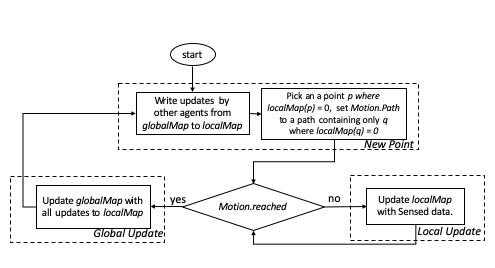
\includegraphics[width=\linewidth]{figs/map_flowchart.png}
%    \caption{Flowchart for a simple solution to 2D distributed mapping problem\vspace{-2mm}}
%    \label{fig:flowmap}
%\end{figure}
%
%
%
%We discuss now discuss how our algorithm implemented $\lgname$ shown in \reffig{mapapp} tackles $\mapprob$. \reffig{flowmap} shows a simple idea for solving this problem for each robot:
%
%The variable $\lmap$ refers to the current mapping $\map_i$ constructed by each robot $i$ using the algorithm. The function $\mathit{MaxExp}$ informally, determines whether there is a grid rectangle in the frontier of the current $\map_i$ . If not, the robot first updates its $\lmap$ from $\gmap$, which is used for sharing the currently computed occupancy maps by all agents so far. The robot then picks a new point in a rectangle known to be unoccupied in its $\lmap$ and follows a path ($\mathit{Motion.Path}$) moving only over grid rectangles known to be unoccupied by its $\lmap$. While the robot hasn't reached the target rectangle, it keeps updating its $\lmap$ with sensed data (occupied and unoccupied rectangles). When it reaches the target, it updates the $\gmap$ from its $\lmap$.
%
%
%

\subsubsection{External (Library) Functions}

% restriction of the world function for sensing. accuracy of sensor statement.
% domain of mapping function for which value is 0 or 1.
% make compatibility a definition instead of lemma.
\subsection{Assumptions}
\label{sec:formal:sensing}

The formal semantics of $\lgname$ is defined under certain timing and system information assumptions. Additionally, given that the application involves interaction with physical plants, we formally state several assumptions about low-level sensing concerns which are abstracted away by $\lgname$.

\subsubsection{Perception}


 % $\map_i(q) = 1$ indicates that according to robot $i$, there is an obstacle in $q$, $\map_i(q) = 0$ indicates that according to robot $i$, $q$ is unoccupied, and $\map_i(q) = -1$ indicates that robot $i$ doesn't have information about $q$.

%We assume that given $\Vec{x} \in q, \forall \Vec{x^\prime} \in q, \sensarea(\Vec{x}) \subseteq \sensarea(\Vec{x^\prime})$.


The sensors used by a robot for perception of the ground truth around it are \emph{Motion.trace} and \emph{Lidar.ldata}, which are \emph{sampled} sensors. Given that $\delta$ is the duration of a \emph{round},

\begin{itemize}
    \item $\mathit{Motion.trace}: [0,\delta] \mapsto \mathit{Pos}$. Given a state $\vs\in Q$ ,  $\forall i \in [N]\vs.\mathit{Motion.trace}_i = \{(t_j, p_j)\}_{j \in [M]}$ where $p_j$ is the position of the robot $i$ at time $t_j$ from the beginning of the round.
    \item  $\mathit{Lidar.ldata} : [0,\delta]\mapsto \mathit{Scan}$. Given a state $\vs\in Q$ , $\forall i \in [N], \vs.\mathit{Lidar.ldata}_i = \{t_j^\prime, l_j^\prime\}_{j^\prime \in M^\prime}$ where $l_j^\prime$ is the LIDAR \emph{scan} at time $t_j^\prime$ from the beginning of the round.
\end{itemize}

\begin{assumption}
    Given a point $p_i$, if there is a corresponding lidar scan $l_i$ when the robot is in $\qfunc(p_i)$, then there is a function $\sensfunc$ such that $\forall q\in Q$ such that $q \in \domain(\sensfunc), \sensfunc(q) = \world_Q(q)$.
\end{assumption}

$\domain(\sensfunc)$ of a robot is defined as its sensing area. This assumption is required to ensure the \emph{Individual soundess} of a mapping updated using LIDAR scan information.
\fTBD{\rg{Need to figure out how to write the assumptions so that the sensor and actuator ports don't do unexpected things during $\delta$ transitions}}
%The sampling frequencies of these sensors may be different, hence the potentially different number of readings, and potentially different timestamps of the readings.

%The function $\mathit{tSync}$ is used to \emph{synchronize} the readings, where we compute a mapping $\mathit{pScan}: \mathit{Pos} \mapsto \mathit{Scan}$, where given a state $\vs\in Q$, a robot $i\in [N]$,  $\vs.\mathit{pscan}_i = \{(p_j^{\prime\prime}, l_j^{\prime\prime})\}_{j^{\prime\prime} \in M ^{\prime\prime}}$, where  $(p, l) \in \vs.\mathit{pscan}_i$ if given $\epsilon > 0$,  $(t,p) \in \vs.\mathit{Motion.trace}, (t^\prime,l )\in \vs.\mathit{Lidar.ldata}_i, |t - t^\prime| \leq \epsilon$.

%The function $\mathit{scanToMap}: \mathit{Scan} \times \mathit{Pos}\mapsto \mathit{GridMap}$, given a position $p_i$ and its corresponding scan $l_i$, computes a quantized domain function $\sensfunc$ for .

%By definition, this returns a \emph{sound} mapping. We stated earlier that the operator $\oplus$ applied to two sound mappings returns a sound mapping. Therefore, given $s_i^\prime$ such that $\mathit{s_i^\prime \in \mathit{trans}(s_i,\mathit{LUpdate})}$,  $s_i^\prime.M.\lmap$ is sound if $s_i.M.\lmap$ is sound.


\begin{definition}
   Given a robot at a position $\Vec{x}\in D, \qfunc{\Vec{x}} = q$, the \emph{sensing area} around $q$ is a function $\sensarea: Q \mapsto 2^{Q}$ where $\forall q^\prime \in \sensarea(q), \sensfunc(q) = \world_Q(q)$.
\end{definition}

%\fTBD{define the data types in the software section}


%The function $\mathit{scanToMap}: \mathit{Scan} \times \mathit{Pos}\mapsto \mathit{GridMap}$, given a position $p_i$ and its corresponding scan $l_i$, computes the quantized domain function$\sensfunc$, in $\sensarea(\qfunc(p_i))$. By definition, this returns a \emph{sound} mapping. We stated earlier that the operator $\oplus$ applied to two sound mappings returns a sound mapping. Therefore, given $s_i^\prime$ such that $\mathit{s_i^\prime \in \mathit{trans}(s_i,\mathit{LUpdate})}$,  $s_i^\prime.M.\lmap$ is sound if $s_i.M.\lmap$ is sound.


\subsubsection{Problem Setup}

A vacuously correct (sound) solution to $\mapprob$ given $D, \qfunc$ and $\world_Q$ is $\forall i \in [N]$, $$\map_i : Q_i \mapsto \left\{0,1\right\}, Q_i = \phi$$ To allow for potentially more interesting solutions than the one stated above, we make the following assumption on the
\begin{assumption}
Initially, each robot $i\in[N]$ starts at a grid rectangle with no obstacle, the sensed area of each robot $i$ is non empty
$\forall i \in [N], \world_Q(q^0_i) = 0\wedge \sensarea(q^0_i) \neq \phi$
where $q^0_i = \qfunc(\pos_0(i))$, and $\pos_0(i)$ denotes the initial position of robot $i$.
\end{assumption}

This ensures that a robot doesn't violate the \emph{Individual soundness} requirement for a correct solution the mapping problem.

\subsubsection{Planning and actuation}

\begin{definition}
    We say that $\Vec{x_n}\in D$ is \emph{accessible} from $\Vec{x_0}$ if there is a \emph{path} $p = \Vec{x_0},\Vec{x_1}, \Vec{x_2},\ldots, \Vec{x_n}$ , such that
    \begin{itemize}
        \item $\forall i \in [0..n],\world_Q(\qfunc{\Vec{x_i}}) = 0$
        \item a robot can move from $\Vec{x_i}$ to $\Vec{x_{i+1}}$ for $i \in [0..n]$, while staying within $\qfunc(\Vec{x_i}) \cup \qfunc(\Vec{x_{i+1}})$.
    \end{itemize}
\end{definition}

A grid rectangle $q\in Q$ is accessible in general, if $\exists \Vec{x}\in D, q = \qfunc(\Vec{x})$ such that $\Vec{x}$ is accessible from either \begin{inparaenum} [(a)] \item the initial position of a robot, or \item another accessible point $\Vec{x^\prime}\in D$. We denote the accessibility of a grid rectangle using a predicate $\Access : Q \mapsto \left\{\mathit{True}, \mathit{False}\right\}$, where $\Access(q) = \mathit{True}$ if its accessible,  $\mathit{False}$ otherwise.
\end{inparaenum}

\begin{assumption}
    The path planner used by the $\lgname$ implementation of the $\dmap$ application returns a path $p = \Vec{x_0},\Vec{x_1}, \Vec{x_2},\ldots, \Vec{x_n}$ , such that the robot can traverse it while staying within $\qfunc(\Vec{x_i})$ for every $\Vec{x_i}\in p$.
\end{assumption}

This assumption can be shown to ensure for the \emph{Safe location} property of a solution, if for robot $i$, the path planner can be restricted to find paths within $\domain(\map_i)$.

%\begin{definition}
%    Given a sound occupancy mapping $\map_i$, the \emph{frontier} of $\map_i$, denoted by $\ff(\map_i)$ is defined as follows:
%    $$ \left\{ q\in Q \mid \Access(q) \wedge \exists q \in \sensarea(\Vec{x}), q \notin \domain(\map_i)\right\} $$
%\end{definition}

%Assume that the planner returns a path if \begin{inparaenum}[(a)] \item the frontier is non-empty \item the grid rectangle picked on the frontier is reachable from the current point \end{inparaenum}. We also constrain the robots to move only on \emph{known} unoccupied grid rectangles, i.e $q\in Q, s_i.M.\lmap[q] = 0$. In implementation, we achieve this by ensuring that the path planner treats all the unknown ($q$ such that $s_i.M.\lmap[q] = -1$) grid rectangles as obstacles as well.


\subsubsection{Synchronization and consistency}
The following are the timing assumptions on $\lgname$ programs.
\begin{assumption} A program step has zero logical execution time.
\end{assumption}
This assumption is reasonable if the time taken to complete a program transition step is negligible compared to $\delta$.  The $\lgname$ middleware ensures that the participating agents begin executing their events synchronously.

\begin{assumption} Shared memory updates are propagated to all agents instantanously.
\end{assumption}
The $\lgname$ middleware uses message passing to implement shared memory, and compared to $\delta$, the time taken to observe a shared memory update as a received message from the time that it is sent is much smaller. We therefore can assume that in this setting, the shared memory semantics of $\lgname$ wherein an update is visible in the next round of program transitions, is a reasonable implementation deliverable. This assumption in this particular example, is required for \emph{Eventual Completeness}, but in other applications, it may be used to correctness.
%$\marginpar{\scriptsize\sayan{MAke this a list of {\bf Assumptions} with discussion on why they hold, or what they mean in English.}}


% \rg{We can \emph{combine} the elements of the set of \emph{local maps}, $\{\map_i\}_{i\in [N]}$ to form a \emph{global} occupancy mapping. }



%
%\begin{definition}
%    Given  $i , j \in [N]$, two proposed occupancy mappings $\map_i: Q_i\mapsto\left\{0,1\right\}$ and $\map_j: Q_j\mapsto \left\{0,1\right\}$, are consistent only if $\forall q \in Q_i \cup Q_j, \map_i(q) = \map_j(q)$.
%\end{definition}




\subsection{Analysis of \dmap}
\label{sec:analysis}


In this section, we present an analysis of the $\lgname$ program for the mapping problem.
% initial states of $\A$.




Consider a state $\vs\in \Reach(\A)$. For $\vs$, the individual soundness, and the soundness requirements of the mapping problem are captured by the following invariants of $\A$ respectively.


\begin{invariant}
\label{ind-sound}
For all $i \in [N]$ $$\forall q_1 \in \domain(\vs.\lmap_i) , \vs.\lmap_i(q) =  \world_Q(q)$$
\end{invariant}

\begin{invariant}
\label{sound}
For all $i \in [N]$, $$\forall q_1 \in \domain(\vs.\gmap_i) , \vs.\gmap_i(q) =  \world_Q(q)$$
\end{invariant}

The consistency requirement of the mapping problem is captured as follows:
\begin{invariant}
\label{consistency}
For all $i,j \in [N]$, for all $q \in \domain(\vs.\lmap_i)\cup \domain(\vs.\lmap_j)$, $$\vs.\lmap_i = \vs.\lmap_j$$
\end{invariant}

We omitted the initialization of the mappings in the presentation of the program in \reffig{mapapp}. From \asum{initval}, for each robot $i$, given its initial state $\vs\in C_0$, $\vs.\lmap_i$ is a sound mapping and $\vs.\gmap_j$ is initialized to be empty, Therefore all initial states satisfy \inv{ind-sound}, and \inv{sound}.


Given $\map_i$, $\map_j$, and $q\in Q_i \cup Q_j$ , let $\map_i(q) = 1$, and $\map_j(q) = 0$. Suppose $\map_i$ is sound, then $\world_Q(q) = 1$, which implies $\map_j$ is not sound. By the same argument, if $\map_j$ is sound, $\map_i$ is not. This implies that $\vs\in C$ has individual soundness only if it also has consistency. Therefore, given $\vs\in C_0$, it satisfies \inv{consistency}.


Suppose, a state of a system $\vs\in C$ satisfies \inv{sound}, \inv{ind-sound} and \inv{consistency} , we now prove that given a transition $(\vs, a, \vs')\in \D$, $\vs'$ also satisfies them. Since these statements are only about \emph{program} variables, $\delta$-transitions don't affect them. Hence, we only need to prove that each event transition preserves these invariants.

\paragraph{NewPoint}
For every robot $i$, $\vs.\gmap_i = \vs'.\gmap_i$. Thus, this event trivially preserves \inv{sound}. So far, we haven't described the \emph{merge} function in detail, but we do so now. Given two mappings $m:Q'\mapsto \mathbb{B}$ and $n:Q''\mapsto \mathbb{B}$, the $\mathit{merge}$ function returns a mapping $\mathit{mn}: Q'\cup Q'' \mapsto \mathbb{B}$ where, \begin{itemize}
      \item for every $q \in Q'\setminus Q''$, $\mathit{mn}(q) = m(q)$
      \item for every $q \in Q''\setminus Q'$, $\mathit{mn}(q) = n(q)$
      \item for every $q \in Q \cap Q''$, $\mathit{mn}(q) = m(q) $
\end{itemize}
If $m$ and $n$ are sound, then $\mathit{merge}(m,n)$ also returns a sound mapping. Given that for every $i\in [N]$, $\vs'.\lmap_i = \mathit{merge}(\vs.\lmap_i,\vs.\gmap_i)$, and by assumption $\vs.\lmap_i$ and $\vs.\gmap_i$ are sound, $\vs'.\lmap_i$ is also sound. Therefore, this event preserves \inv{ind-sound}.

Now suppose that \inv{consistency} is not preserved, i.e. there are robots  $i, j \in [N]$, and a common $q \in \domain(\vs'.\lmap_i)\cap\domain(\vs'.\lmap_j)$, such that $\vs'.\lmap_i[q] \neq \vs'.\lmap_j[q]$. However, since $\vs'$ satisfies \inv{ind-sound}, we have proved that this event preserves \inv{consistency} by contradiction.

\paragraph{LUpdate}
Again, for every robot $i$, $\vs.\gmap_i = \vs'.\gmap_i$. Thus, this event trivially preserves \inv{sound}.

As before, we can prove as that since \emph{LUpdate} preserves \inv{ind-sound}, it also preserves \inv{consistency}.

\paragraph{GUpdate}
Since for every robot $i$, $\vs.\lmap_i$ and $\vs.\gmap_i$ are sound, by definition of \emph{merge},  $\vs'.\gmap_i$ is also sound. Therefore, this event preserves \inv{sound}. \emph{GUpdate} preserves \inv{ind-sound} trivially as it doesn't modify $\vs.\lmap_i$, and as a result, it also preserves \inv{consistency}.


%\begin{lemma}
%    \label{ext}
%    Given a robot $i$, suppose the mapping $\map_i:Q_i \mapsto \mathbb{B}$, where $Q_i\subseteq Q$, is sound. Suppose further, that the robot $i$ is is within $q'\in Q$. Consider a mapping, $\map^\prime_i: Q_i \cup \sensarea(q') \mapsto \mathbb{B}$
%    such that, $\forall q\in Q_i, map^\prime_i(q) = map_i(q)$
%    and $\forall q \in \sensarea(q'), \map^\prime_i(q) = \sensfunc(q)$. Then, $\map'_$
%\end{lemma}
%
%The proof for this is straightforward and follows from the definition of $\map^\prime_i$ combined with \defn{soundness}.
%
%Recall from the definition of the sensing area of a robot $i$ at $\pos(i)$, that it can reliably compute the ground truth mapping $\world_Q$ for all $q \in \sensarea(\pos(i))$. This lemma essentially states that given a sound occupancy mapping $\map_i$, it can be used to compute to another \emph{sound} occupancy mapping $\map^\prime_i$ by setting the values of $\map^\prime_i(\sensarea(\pos(i)))$ to the ground truth function.

%Given a mapping $\map_i$, $\domain(\map_i)$ denotes $ Q_i \subset Q$, such that $\forall q \in Q_i \map_i(q) = 0 \vee \map_i(q) = 1$.


%$Given two sound maps $\lmap$ and $\gmap$, $\lmap \oplus \gmap$ corresponds to a combined map construction as outlined in \defn{cons}, and is sound. The event \emph{NewPoint} doesn't modify $s_i.M.\lmap$ further, and therefore, $\lmap$ remains \emph{sound} during the execution of this event.

%\begin{definition}
%    We say that $\Vec{x_n}\in D$ is \emph{reachable} from $\Vec{x_0}$ if there is a \emph{path} $p = \Vec{x_0},\Vec{x_1}, \Vec{x_2},\ldots, \Vec{x_n}$ , such that
%    \begin{itemize}
%        \item $\forall i \in [0..n],\world_Q(\qfunc{\Vec{x_i}}) = 0$
%        \item a robot can move from $\Vec{x_i}$ to $\Vec{x_{i+1}}$ for $i \in [0..n]$, while staying within $\qfunc(\Vec{x_i}) \cup \qfunc(\Vec{x_{i+1}})$.
%    \end{itemize}
%\end{definition}
%
%A grid rectangle $q\in Q$ is reachable in general, if $\exists \Vec{x}\in D, q = \qfunc(\Vec{x})$ such that $\Vec{x}$ is reachable from either \begin{inparaenum} [(a)]
%                                                                                                                                                   \item the initial position of a robot, or \item another reachable point $\Vec{x^\prime}\in D$. We denote the reachability of a grid rectangle using a predicate $\mathit{Reach} : Q \mapsto \left\{\mathit{True}, \mathit{False}\right\}$, where $\mathit{Reach}(q) = \mathit{True}$ if its reachable,  $\mathit{False}$ otherwise.
%\end{inparaenum}
%
%\begin{definition}
%    Given a sound occupancy mapping $\map_i$, the \emph{frontier} of $\map_i$, denoted by $\ff(\map_i)$ is defined as follows:
%    $$ \left\{ q\in Q \mid Reach(q) \wedge \exists q \in \sensarea(\Vec{x}), q \notin \domain(\map_i)\right\} $$
%\end{definition}


\begin{theorem}
    For the system of robots $[N]$ executing the $\lgname$ program shown in \reffig{mapapp}, the shared variable $\gmap$ represents a sound mapping of the domain $Q$.
\end{theorem}

%\begin{lemma}
%    \label{ext}
%    Suppose robot $i$ is at $\pos(i)\in D$, and $\exists(q^\prime)\in \sensarea(\pos(i))$,
%    s.t $\map_i(q) = -1$. Consider a mapping, $\map^\prime_i:Q \mapsto \left\{-1,0,1\right\}$
%    such that, $\forall q\in Q \setminus \sensarea(\pos(i)), map^\prime_i(q) = map_i(q)$
%    and $\forall q \in \sensarea(\pos(i)), \map^\prime_i(q) = \world_Q(q)$.
%    Then, $\map^\prime_i(q)$ is sound if $\map_i$ is sound.
%\end{lemma}
%
%The proof for this is straightforward and follows from the definition of $\map^\prime_i$ combined with \defn{soundness}.
%
%Recall from the definition of the sensing area of a robot $i$ at $\pos(i)$, that it can reliably compute the ground truth mapping $\world_Q$ for all $q \in \sensarea(\pos(i))$. This lemma essentially states that given a sound occupancy mapping $\map_i$, it can be used to compute to another \emph{sound} occupancy mapping $\map^\prime_i$ by setting the values of $\map^\prime_i(\sensarea(\pos(i)))$ to the ground truth function.
%
%\begin{definition}
% We say that $\Vec{x_n}\in D$ is \emph{reachable} from $\Vec{x_0}$ if there is a \emph{path} $p = \Vec{x_0},\Vec{x_1}, \Vec{x_2},\ldots, \Vec{x_n}$ , such that
%\begin{itemize}
%\item $\forall i \in [0..n],\world_Q(\qfunc{\Vec{x_i}}) = 0$
%\item a robot can move from $\Vec{x_i}$ to $\Vec{x_{i+1}}$ for $i \in [0..n]$, while staying within $\qfunc(\Vec{x_i}) \cup \qfunc(\Vec{x_{i+1}})$.
%\end{itemize}
%\end{definition}
%
%A grid rectangle $q\in Q$ is reachable in general, if $\exists \Vec{x}\in D, q = \qfunc(\Vec{x})$ such that $\Vec{x}$ is reachable from either \begin{inparaenum} [(a)]\item the initial position of a robot, or \item another reachable point $\Vec{x^\prime}\in D$. We denote the reachability of a grid rectangle using a predicate $\mathit{Reach} : Q \mapsto \left\{\mathit{True}, \mathit{False}\right\}$, where $\mathit{Reach}(q) = \mathit{True}$ if its reachable,  $\mathit{False}$ otherwise.
%\end{inparaenum}
%
%\begin{definition}
%    Given a sound occupancy mapping $\map_i$, the \emph{frontier} of $\map_i$, denoted by $\ff(\map_i)$ is defined as follows:
%    $$ \left\{ q\in Q \mid Reach(q) \wedge \exists q \in \sensarea(\Vec{x}), \map_i(q) = -1\right\} $$
%\end{definition}
%
%Given a sound occupancy mapping $\map_i$, another sound mapping $\map_i^\prime$ can be constructed as shown in \lem{ext}. Taken in conjunction with our assumption on the initial positions of each robot, this leads to a strategy for computing sound occupancy mapping functions. Further, given a set of sound mappings $\left\{\map_i\right\}_{i\in[N]}$, we can construct a sound mapping $\map$ from them as follows :
%

%
%

%
%
%

% restriction of the world function for sensing. accuracy of sensor statement.
% domain of mapping function for which value is 0 or 1.
% make compatibility a definition instead of lemma.


\subsection{Implementation of Modules}

\paragraph{Sound Mapping from Synchronized Sensor Data~(ScanToMap).}
To generate a 2D map from the scan data,
it is required to synchronize the current vehicle position and the Lidar scan data.
An existing solution is to filter the time stamps of both sensor data streams
and only choose pairs of data within a given time difference threshold $\epsilon$.
This can be achieved by \texttt{ApproximateTimeSynchronizer} in the ROS package named \texttt{message\_filter}.
The frequency of the synchronized data is then limited to the sensor with the lowest frequency.
In our simulation, the lowest frequency is 100 Hz for sensing the vehicle position and sufficient for updating the map.

The Lidar scan data provided in the tool chain are pairs of a distance to obstacles and an angle with respect to the heading angle of the vehicle.
To implement ScanToMap, it is then straightforward to compute the positions of obstacles and mark occupied grid rectangles,
and to mark a rectangle obstacle free is to simply check if all four corners of a grid rectangle are covered in the scan.
The time difference $\epsilon$ however can introduce an error between real and perceived distances to obstacles.
Reducing this error is beyond the scope of this work.
Our implementation of ScanToMap therefore may falsely mark a grid rectangle as occupied when obstacles are in nearby grids.

\paragraph{Path to Frontier~(PathToFrontier).}
In the \toolname tool chain, several path planning algorithms are already available.
We particularly select the Rapidly exploring Random Tree with near neighbor search and rewiring tree~(RRT*) algorithm.
It is able to avoid obstacles and is fine tuned to the car model for simulation.
Our implementation hence only needs to choose a point in frontier grid rectangles and provide the positions of obstacles.
To choose such a point, a basic solution is to use Breadth-First Search~(BFS) on the map and seek for a unexplored grid rectangle.
BFS ensures that either all reachable grid rectangles are marked,
or there are connected unoccupied rectangles to an unexplored rectangle, and hence a path must exist.
Nonetheless, it does not guarantee that the underlying path planner can always find a path because,
for instance, the car is incapable of make sharp turns.
Our soundness claim still holds under such circumstance, but we may not be able to progress even when paths to frontier exist.

\section{Examples showcasing features of $\lgname$ language and simulator}
\label{sec:experims}
The $\lgname$ simulator provides the user a way to test and  debug application programs with different and heterogeneous physics models. We present three case studies to demonstrate some of the key features of the $\lgname$ language and its  simulator.

\subsection{Platooning}
%end to end
\label{sec:platooning}
Figure~\ref{fig:platooningapp} shows the $\lgname$ program for a simplified platooning protocol for vehicles on a single lane. The position of successive vehicles is communicated through  {\bf allread} shared variable $\mathit{x}$. The  goal is to maintain a minimal  \emph{safe} separation  of $5$ meters between any two consecutive cars. For the sake of simplicity, here the leading car  has a preprogrammed behavior (it sets its acceleration to $2$ or $-2$ every $100$ rounds); in a more realistic deployment this behavior could be based on speed limits or other traffic. 
%The motion controller for the car has bounds on highest and lowest velocities allowed. 
Every other car in the platoon with pid $i$ sets the actuator, namely, its acceleration $\mathit{Motion.xacc}$ based on its distance from the car with pid $i+1$; slowing down when the separation is less than the $\mathit{threshold}$ of $8$ meters, accelerating otherwise. 
%The cars communicate through the \emph{allread} variable $\mathit{pos}$, which they update every time they execute the event \emph{SetAcc}, or, as the semantics dictates, every $\delta$ time units.

\begin{figure}[ht!]
\begin{mdframed}
    \noindent
    \begin{center}
        \scriptsize
        \two{0.4}{0.6}
        {\lstinputlisting[language=koordNums,firstline=1,lastline=14,frame=none]{code/platooning3.tex}}
        {\lstinputlisting[language=koordNums,firstline=15,frame=none,firstnumber=15]{code/platooning3.tex}} 
    \end{center}
\end{mdframed}
    \caption{$\lgname$ program for robot $i$ in a platoon to adjust its $x$ acceleration accordingly .}
    \label{fig:platooningapp}
\end{figure}

%\sayan{Why some ifs have ( ) others do not? Let us use x as position like in lineform.}
Recall that the synchronous semantics of $\lgname$ implies that in each round the participating vehicles update their modes and accelerations based on the positions of others updated from the last round. These updates can happen in arbitrary order but all in zero logical execution time. The resulting decisions affect the actuation ($\mathit{Motion.xacc}$) for a period of $\delta$ time, before the execution of the next round. 

\reffig{platoon} shows the simulator generated position $x$ vs $\mathit{time}$ plots for different values of $\delta$, for four vehicles.

\begin{figure}[ht!]
\begin{minipage}{0.5\textwidth}
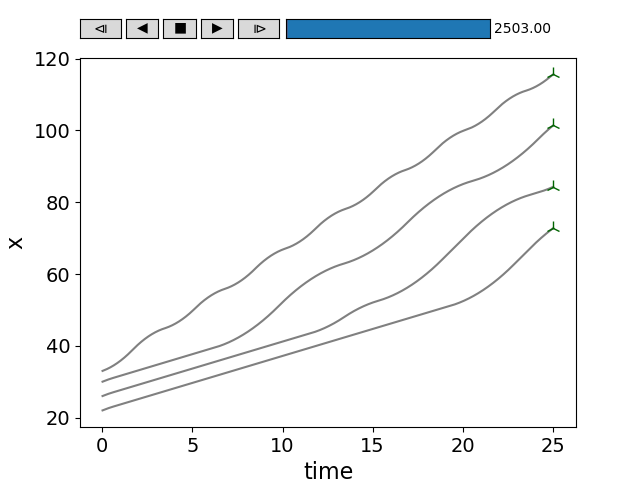
\includegraphics[width=.5\textwidth]{figs/braking_acc.png}\hfill
%\includegraphics[width=.3\textwidth]{figs/Platooning_2.png}}\hfill%
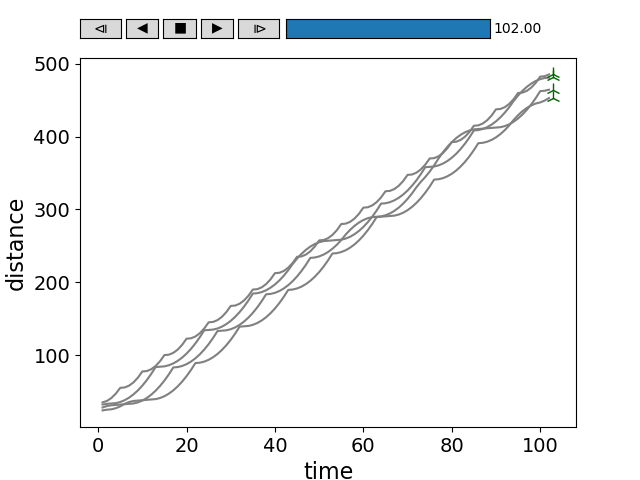
\includegraphics[width=.5\textwidth]{figs/braking_bad.png}
\end{minipage}%
	\caption{\small {Platoon of four cars. \emph{Left} for $\delta = 0.01$, the cars eventually get to safe separations, while reacting to the first car changing its acceleration periodically} and \emph{Right} for $\delta = 0.1$, this shows an unsafe execution where the simulation stops upon a collision.}
\label{fig:platoon}
\end{figure}

%FIGURE OUT THE VERIFICATION. 
% While the simulator enables quick cycles of development and testing, the verification component, as stated earlier, allows the user to tune the conditions under which the program exhibits desired behavior. 
 A \emph{correct} program should ensure that at no point, the separation along the $x$-axis between two of agents is less than the required safe distance ($8$ m).  Note, that the variable $\emph{threshold}$ needs to be set to be higher for larger values of the round duration $\delta$. If $\delta$ is too long, then the cars will not slow down even when the separation between then might have become less than the $\mathit{threshold}$. We verified using the $\kbmc$ tool that \emph{Platoon} is safe for four cars when $\delta$ is small enough and has potential unsafe behaviors otherwise. \reffig{platoon}(Right) shows the $x$ vs $\mathit{time}$ for a counterexample with  $\delta$ is too long. For a threshhold value of $8.0$, required minimum separation of $5.0$, for $\delta = 0.01$ $\kbmc$  showed that the program was safe for 10 rounds starting at an initial configuration where each car $i$ is at a distance of 6.0 from the car $\mathit{i}+1$, For $\delta = 0.1$ $\kbmc$ showed that the program was unsafe. 
 
%\sayan{Last 2 sentences are not clear. What changed between the safe and the unsafe scenarios? Explain clearly. Put a box around the code.}

\subsection{Swarm formation}
%portability
\label{sec:formation}
We used $\lgname$ to implement several standard pattern formation protocols like the  \emph{Lineform} app from the Introduction.  
%
%\begin{figure}[ht!]
%	\label{fig:lineform}
%	\noindent
%	\begin{center}
%		\scriptsize
%		\two{0.4}{0.6}
%		{\lstinputlisting[language=xyzNums,frame=none]{code/lineform.tex}}
%		{ \vspace{0.1in}
%                        $x_{t+1} = Ax_{t}$, where \\
%			$x_0$: vector of initial position of agents, \\
%			$x_{t}$: position vector at time $t$, and \\
%		        $A$: is the \emph{transition matrix}, for lineform  \\
%                  
%			$A  = \left[ \begin{array}{ccccc}
%			0 & 0 & 0 & 0 & 0\\
%			\frac{1}{2} & 0 & \frac{1}{2} & 0 & 0\\
%			0 & \frac{1}{2} & 0 & \frac{1}{2} & 0  \\
%			0 & 0 & \frac{1}{2} & 0 & \frac{1}{2} \\
%			0 & 0 & 0 & 0 & 0\\			
%			\end{array}\right]$
%			}
%	\par
%        
%	\end{center}
%	\caption{\small $\lgname$ program for line formation ({\em Left}) and its mathematical counterpart in robotics and control textbooks ({\em Right}).}
%\end{figure}
%
The shared \emph{allread} variable $x$ is used by the agents to communicate their position to the other robots. The function \emph{mid} computes the centroid of a list of vectors.
% In the case of 3D shape formation,  
%is a part of the library functions provided for the data type \emph{pos}; where 
%$$\mathit{midpoint}(p_1,p_2,\ldots,p_n) = pos(\frac{\Sigma_n p_i.x}{n},\frac{\Sigma_n p_i.y}{n},\frac{\Sigma_n p_i.z}{n}) $$.


With the addition of an explicit neighbor relation, the \emph{Squareform} app as shown in \reffig{squareform} can be used to generate a rhombus shape in the plane formed by four extremal points. The code defines a local variable $nbrs$ which is a static list of list of integers, where the $i$th element is a list of the $\mathit{pid}$s of the neighbors of the agent with $\mathit{pid}$ $i$. The list of $\mathit{pid}$s of the extremal points is stored in a list of integers called $\mathit{corners}$. If the agent $\mathit{pid}$ is not in $\mathit{corners}$, then it moves to the mid point of all its neighbors. \footnote{We omit the actual initialization of the variables $\mathit{nbrs}$ and $\mathit{corner}$, as it depends on the simulation parameters.}

\begin{figure}[ht!]
\begin{mdframed}
    \noindent
    \begin{center}
        \scriptsize
        \two{0.4}{0.6}  {\lstinputlisting[language=koordNums,firstline=1,lastline=10,frame=none]{code/shapeform.tex}}
{\lstinputlisting[language=koordNums,firstline=11,frame=none,firstnumber=11]{code/shapeform.tex}}
    \end{center}
\end{mdframed}
    \caption{$\lgname$ application forming a shape in 3D defined by the static corners.}
    \label{fig:squareform}
\end{figure}

\reffig{shapeplots} shows two screenshots of the 3d-simulation for the \emph{Shapeform} app with 25 agents. Here the $\mathit{Motion}$ controller used is a simple drone model. Instead of the $\mathit{mid}$ function, other operators on the positions of the neighboring agents could be applied to create different swarming protocols. In addition, using the scripting technique for the leading vehicle in $\mathit{Platoon}$, the swarming robots can be guided to move in formation.


\subsection{Distributed task allocation}
\label{sec:task}
 \reffig{taskapp} shows the distributed task allocation application written in $\lgname$. Distributed task allocation is challenging as it involves mutual exclusion as well as construction of de-conflicted paths to task locations. Tasks can be abstractions for real location-based objectives like package delivery, surveillance, or fire-fighting. 

We implement a  task allocation strategy using shared variables for coordination. Mutual exclusion is always an essential feature when shared variables are involved. $\lgname$ provides a locking mechanism using the keyword $\mathit{atomic}$, which the $\mathit{Assign}$ event uses to update the shared list of tasks $\mathit{taskList}$ safely. 

Here the motion module implements Dubin-like vehicle models for the agents, and RRT-based path planning to avoid static obstacles specified in map. \reffig{taskplots} shows two screenshots of a $\mathit{Task}$ application simulations. 

\begin{figure}[h!]
\begin{minipage}{0.5\textwidth}
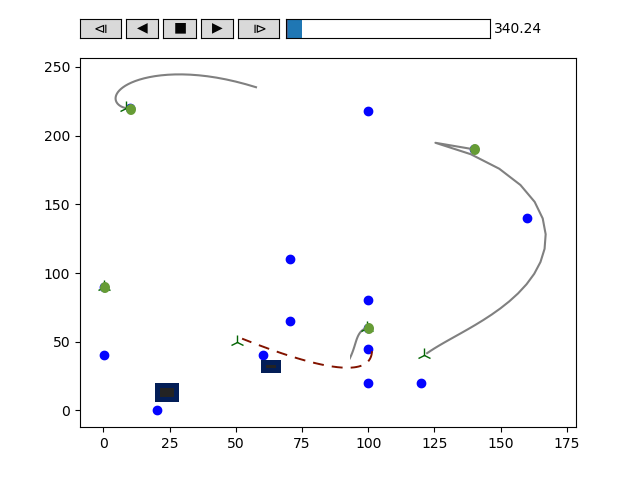
\includegraphics[width=.5\textwidth]{figs/task2.png}\hfill
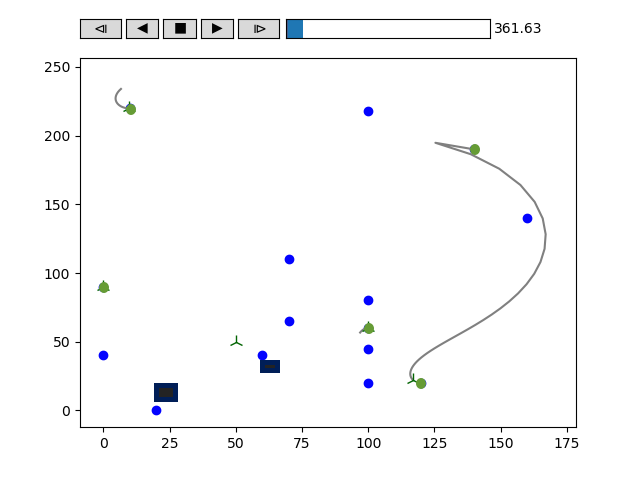
\includegraphics[width=.5\textwidth]{figs/task1.png}\hfill%
%\includegraphics[width=.3\textwidth]{figs/Platooning_2.png}}\hfill%
\end{minipage}%
\caption{\small The grey trails represent the positions of the five agents in the last $150$ time units; task locations of the incomplete tasks (blue), completed tasks (green), static obstacles (black), currently computed infeasible path (dashed red).}
\label{fig:taskplots}
\end{figure}

We could  easily replace the $\mathit{Motion}$ automaton (consequently, the dynamical model) of any of the agents, and run the same code. Using different control parameters, and path planning parameters for the same motion automaton we obtain different statistics for task completion and distance traversal as depicted in in \reffig{completionstats}. This heterogeneity and portability can be useful for coordinating the same application between different hardware platforms. We ran the task application for various configurations of cars (moving in 2d) and quadcopters (moving in 3d) for the task application, and present some completion statistics below. The agents performed 25 tasks, with three obstacles. An agent (car or quadcopter) is considered to have reached a task location if the $x$ and $y$ coordinates of the task are within a specified minimum distance of the current $x$ and $y$ coordinates of the agent.

 For all agents operating with the same motion automaton and dynamics model, we observed that conflict resolution took more time with more agents, as expected (\reffig{completionstats}). The completion time remained relatively stable. The maximum and minimum distances travelled were relatively closer with more robots. However, all these results were affected by the non-determinism in choice of paths and tasks by the agents, and their previous relative positions at the moment of choosing the next task as well. 
 
 
\begin{wrapfigure}{r}{0.26\textwidth}
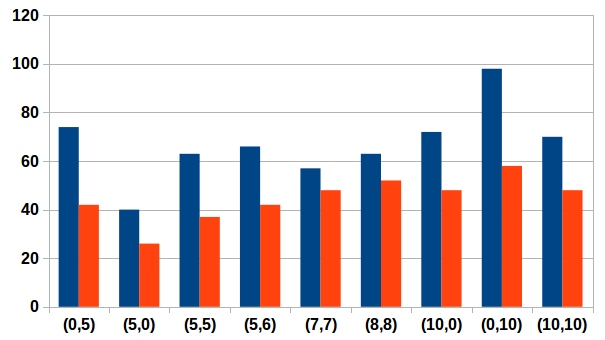
\includegraphics[scale=0.3]{figs/completion.png}\hfill
\caption{\small Completion time (orange) and conflict resolution time (blue)  for different agent configurations (quadcopters, cars). }
\label{fig:completionstats}
\end{wrapfigure}

These results demonstrate a capability of covering various scenarios with different levels of heterogeneity and coordination.
 

\section{Conclusions and Future Work}


Our vision is to provide a programming methodology to enable programming safe distributed cyber-physical applications without the need of complete domain expertise in all related areas such as control theory, robotics motion control, and network protocols.
To this end, we demonstrated how \lgname application developers can write succinct multi-robot applications involving distributed coordination,
different types of sensing and actuation, and path planning in three case studies, each of which requires only preliminary knowledge
in shared memory and basic concurrency control via atomic blocks and assumptions on sensor and actuator ports of controllers.
V\&V engineers with deep understanding in distributed computing are able to focus on formally analyzing invariant properties of \lgname programs via symbolic execution, and roboticists can validate the feasibility of assumptions by examining rigorously defined proof obligations.

We acknowledge the fact that our \portasum based abstractions may not cover various vastly different types of robots.
\K semantics framework can allow us to extend our language to tailor to specific robot types on demand
while retaining the same framework for formal analysis. We also plan to extend this work to include specification and verification of progress properties under fairness constraints for \lgname applications.


%% Acknowledgments
\begin{acks}                            %% acks environment is optional
                                        %% contents suppressed with 'anonymous'
  %% Commands \grantsponsor{<sponsorID>}{<name>}{<url>} and
  %% \grantnum[<url>]{<sponsorID>}{<number>} should be used to
  %% acknowledge financial support and will be used by metadata
  %% extraction tools.
  This material is based upon work supported by the
  \grantsponsor{GS100000001}{National Science
    Foundation}{http://dx.doi.org/10.13039/100000001} under Grant
  No.~\grantnum{GS100000001}{nnnnnnn} and Grant
  No.~\grantnum{GS100000001}{mmmmmmm}.  Any opinions, findings, and
  conclusions or recommendations expressed in this material are those
  of the author and do not necessarily reflect the views of the
  National Science Foundation.
\end{acks}


%% Bibliography
\bibliography{cyphyhouse,sayan1}


%% Appendix
\appendix


\section{Code and Figures}
\chiao{Appendix should not be included for PLDI and should be provided separately as supplementary materials.
We just put figures and code here for now to count the pages.}


\subsection{Distributed Task Allocation}


\begin{figure}[h!]
    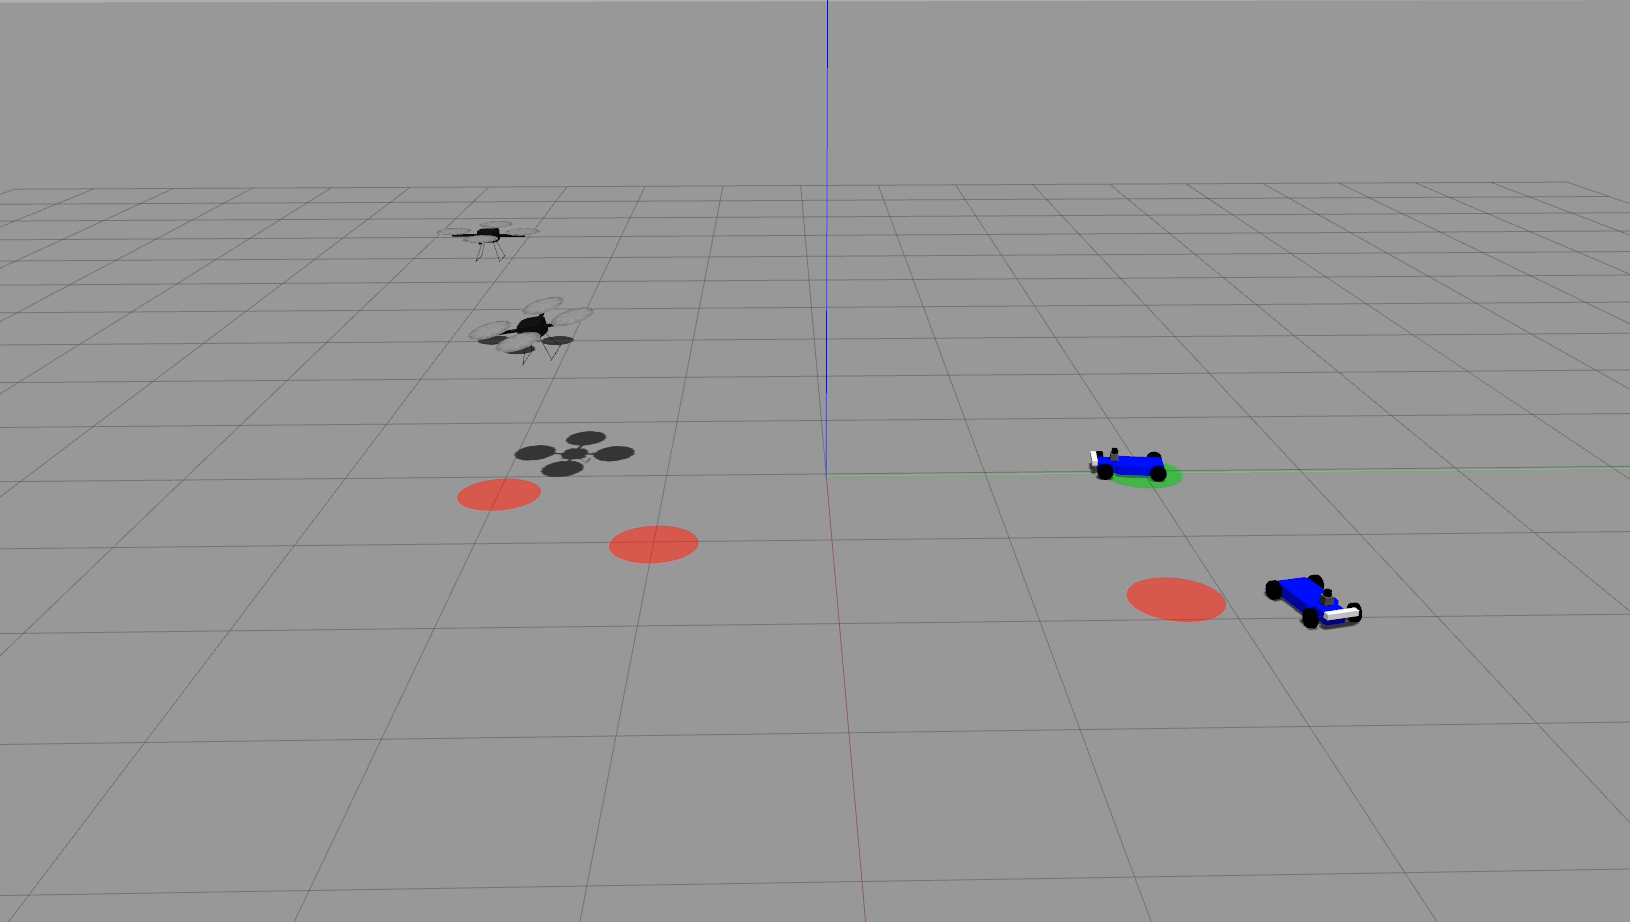
\includegraphics[width=\columnwidth]{figs/taskalloc_w_marker.png}

    \caption{Screenshot in the simulation of Distributed Task Allocation}
\end{figure}

\begin{figure*}[t]
    \two{0.4}{0.6}
    {
    \lstinputlisting[language=NumKoord, lastline=17]{code/taskalloc.tex}
    }
    {
    \lstinputlisting[language=NumKoord, firstline=18, firstnumber=18]{code/taskalloc.tex}
    }

    \caption{Distributed Task Allocation}
\end{figure*}


\subsection{Distributed Mapping Problem}
\sayan{
    Informally, the problem requires a set of robots to collaboratively mark the position of static \emph{obstacles} within a given area $D$, which any robot should avoid while moving in $D$.The key difference between distributed SLAM and this application is that we assume that the robots know their \emph{global coordinates} within the area of deployment. They are only attempting to map the static obstacles within this area. We currently assume that the only sensors available for sensing obstacles are LIDAR based, and the robots are constrained to move in a 2-D space.
}

\subsection{\dmap Application}

\reffig{flowmap1} shows a simple idea for solving the mapping problem problem for each robot, and \reffig{mapapp} shows our solution to $\dmap$ written using $\lgname$, a high level language with native support for multi-robot systems designed to interact with a physical environment. The design of solution to the mapping problem in \reffig{flowmap1} captures an occupancy map of the 2D space in a variable $\gmap$. \reffig{flowmap}. The variable $\lmap$ is a local mapping constructed by each robot $i$ using sensors, and information from other robots shared via $\gmap$. The robot first updates its $\lmap$ from $\gmap$, which stores the currently computed occupancy map \emph{by all robots}.  The robot then picks a new point in the grid known to be unoccupied in its $\lmap$ and follows a path ($\mathit{Motion.Path}$) moving only over grid rectangles known to be unoccupied by its $\lmap$. While the robot hasn't reached the target rectangle, it keeps updating its $\lmap$ with sensed data (occupied and unoccupied grid points). When it reaches the target, it updates the $\gmap$ with new data from its $\lmap$.


\begin{figure}[!htbp]
    \centering
    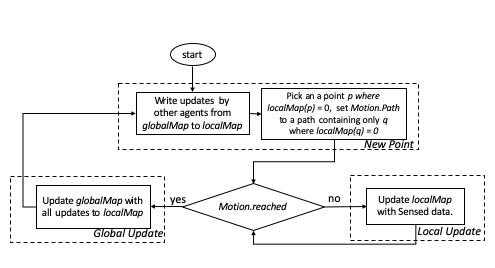
\includegraphics[width=\linewidth]{figs/map_flowchart.png}
    \caption{Flowchart for a simple solution to 2D distributed mapping problem\vspace{-2mm}}
    \label{fig:flowmap1}
\end{figure}

 An \emph{allwrite} variable is a shared variable which all robots can read from and write to. The shared \emph{allwrite} variable $\gmap$ is used to construct a shared map of obstacles within the domain $D$, and has type $\mathit{GridMap}$, which is a 2-D array representing a grid over $D$. The \emph{local} variable $\lmap$ represents each robot's \emph{local} knowledge of the domain $D$, and has the same type as $D$. A robot executing the \emph{NewPoint} event, first updates a \emph{local variable} $\lmap$ from the shared variable $\gmap$, using a combination operator $\oplus$, described in more detail in \refsect{prelims}. $\lgname$ allows the user to use library functions, like the $\mathit{findPath}$ function, which uses a path planner to find a path to a point while avoiding a set of \emph{obstacles}. The point is picked using the $\mathit{pickFrontierPos}$ function which is a user defined function implemented in $\lgname$. The details of the path planner, and how the point is picked are discussed in and \refsect{prelims} \refsect{experiments}.

In $\dmap$, there are two modules \emph{Motion} and \emph{Lidar} which provide interfaces to different sensors and actuators on the robot. The $\mathit{Lidar.ldata}$ sensor module is used to read the LIDAR scan of the actual robot. In the \emph{NewPoint} event, the controller driving the robot directs it along a path set at the actuator port $\mathit{Motion.path}$. The sensor port $\mathit{Motion.psn}$ gives the position of the robot (in a fixed coordinate system) and $\mathit{Motion.reached}$ indicates whether the controller is active or inactive.

The $\lgname$ program corresponding to this solution has three \emph{events}: \emph{NewPoint, LUpdate, GUpdate}. Each robot in the system runs an instance of the \emph{same} program. At runtime, the $\lgname$ program executes within the runtime system of a single robot, or a collection of programs execute on different robots. The $\lgname$ language semantics ensures that the execution of the program in the distributed system occurs in \emph{rounds} of duration $\delta$. In each round, each robot executes the statements in the effect(\textbf{eff}) of at most one \emph{enabled} event : an event whose precondition(\textbf(pre)) is satisfied. If no event is enabled, the robot does nothing. Before the next round of execution, the robot may continue to interact with the physical environment as directed by its controllers. The $\lgname$ semantics imposes a synchronous model of execution for $\lgname$ programs for multi-robot systems and its implementation in CyPhyHouse toolchain ensures that this schedule is maintained by the multi-robot system executing the $\lgname$ program, despite potentially imprecise synchronization of local clocks.

\begin{figure}[!htbp]
    \noindent
    \begin{center}
        \lstdefinelanguage{dmap}[]{NumKoord}{
            morekeywords=[2]{
                Grid, GridMap,
                Scan,
            }
        }
        \two{0.33}{0.62}
        {\lstinputlisting[language=dmap,firstline=1,lastline=22]{code/mapapp.tex}}
        {\lstinputlisting[language=dmap,firstline=23,firstnumber=23]{code/mapapp.tex}}
    \end{center}

    \caption{$\lgname$ code for robot $i$ for the 2D distributed mapping application.}
    \label{fig:mapapp}
\end{figure}

In the design of the $\dmap$ application, we employ the use of \emph{sampled} sensors, which is essentially a sequence of timestamped sensor readings between rounds. The \emph{LUpdate} event can occur while each robot is traversing a path and hasn't reached the final destination, during which the robot uses a sampled sensor reading of the positions $\mathit{Motion.trace}$, of type $\mathit{PosStamped}[]$, which denotes an array of timestamped positions; and a sampled sensor reading of LIDAR scans $\mathit{Lidar.ldata}$ of type $\mathit{ScanStamped}$, which denotes an array of timestamped LIDAR scans. These sampled sensor readings are then synchronized to associate a LIDAR scan with a position.

Mutual exclusion is an essential feature required in a distributed system with shared variables. The robot updates the shared variable $\gmap$ in the event \emph{GUpdate} using the value of its $\lmap$, which may have been updated with newly detected obstacles


\end{document}
